%\documentclass{IEEEtran}
\documentclass{article}

%\IEEEoverridecommandlockouts
% The preceding line is only needed to identify funding in the first footnote. If that is unneeded, please comment it out.
\usepackage{capt-of}
\usepackage{cite}
\usepackage[table]{xcolor}
\usepackage[onehalfspacing]{setspace}
\usepackage{longtable}
\usepackage{geometry}
\usepackage{blindtext}
\usepackage{amsmath,amssymb,amsfonts}
\usepackage{setspace}
\usepackage{algorithmic}
\usepackage{graphicx}
\usepackage{textcomp}
\usepackage{hyperref}
\usepackage[utf8]{inputenc}
\usepackage{subfigure}
\usepackage{svg}
\usepackage{amsmath}
\usepackage{booktabs}
\usepackage{multirow,tabularx}
%\usepackage{subfig}
%% Rechtecke um Text %%
\usepackage{mdframed}
%% eigene packages
\usepackage{float}
\usepackage{subfiles}
\usepackage[T1]{fontenc}
\usepackage{listings}
\usepackage{color}
\usepackage[english,ngerman]{babel}

	
\usepackage{wrapfig}
\geometry{
	left=3cm,
	right=3cm,
	top=2cm,
	bottom=2cm,
	bindingoffset=5mm
}

\definecolor{dkgreen}{rgb}{0,0.6,0}
\definecolor{gray}{rgb}{0.5,0.5,0.5}
\definecolor{mauve}{rgb}{0.58,0,0.82}

\lstset{frame=tb,
	language=Java,
	aboveskip=3mm,
	belowskip=3mm,
	showstringspaces=false,
	columns=flexible,
	basicstyle={\small\ttfamily},
	numbers=none,
	numberstyle=\tiny\color{gray},
	keywordstyle=\color{blue},
	commentstyle=\color{dkgreen},
	stringstyle=\color{mauve},
	breaklines=true,
	breakatwhitespace=true,
	tabsize=3
}

\newsavebox{\fminipagebox}
\NewDocumentEnvironment{fminipage}{m O{\fboxsep}}
{\par\kern#2\noindent\begin{lrbox}{\fminipagebox}
		\begin{minipage}{#1}\ignorespaces}
		{\end{minipage}\end{lrbox}%
	\makebox[#1]{%
		\kern\dimexpr-\fboxsep-\fboxrule\relax
		\fbox{\usebox{\fminipagebox}}%
		\kern\dimexpr-\fboxsep-\fboxrule\relax
	}\par\kern#2
}

\def\BibTeX{{\rm B\kern-.05em{\sc i\kern-.025em b}\kern-.08em
    T\kern-.1667em\lower.7ex\hbox{E}\kern-.125emX}}

\renewcommand{\figurename}{Abbildung}
\renewcommand{\contentsname}{Inhaltsverzeichnis}
\begin{document}

\begin{titlepage}
	\begin{figure}[H]
		\centering
		\subfigure{
			
\includegraphics[width=.4\textwidth]{pictures/uol_logo.png}
		}        
	\end{figure}
	
	\begin{center}
		\large{\textbf{Konzept und Ansatz einer Wertschöpfungskette für die Erkennung und Bereitstellung neuer Fahrumfänge für intelligente Fahrzeuge}}\\
		\large Bachelorarbeit
	\end{center}
	\vfill
	\begin{center}
		\large{
			An der\\
			Carl von Ossietzky Universität Oldenburg\\
			Studiengang Wirtschaftsinformatik\\
			
			\vspace{1cm}
			Vorgelegt von Linus Hestermeyer\\ 
			\textit{linus.hestermeyer@gmail.com}\\
			Matr.Nr.: 4087097\\
			\vfill
			Erstprüfer: Prof. Dr. Frank Köster\\
			Zweitprüfer: Dipl.-Inform. Gerald Sauter\\
			\vfill
			\noindent
			Oldenburg, den \today
		}
	\end{center}
\end{titlepage}
\clearpage
\newpage
\thispagestyle{empty}
\null
\newpage
\thispagestyle{empty}
\null
\begin{huge}
	\textbf{Vorwort}\\\\
\end{huge}
Diese Arbeit entstand im Rahmen meines Wirtschaftsinformatik Studiums an der Carl von Ossietzky Universität Oldenburg.\\\\
Mein Besonderer Dank gilt meinen Betreuern Gerald Sauter und Prof. Dr. Frank Köster für die stetige fachliche Betreuung und Hilfe bei der Erstellung der Arbeit und des Prototypen. Der initiale Gedankenaustausch über die Thematik und die gemeinsame Anpassung des Kernthemas der Arbeit haben das Ergebnis erst möglich gemacht.\\\\
Selbstverständlich gilt mein Dank auch meinen Eltern Andrea und Andreas sowie meinen Geschwistern Johanna und Lukas, die mich bei der Entwicklung meiner fachlichen und beruflichen Laufbahn stets unterstützt haben.\\\\
Nicht zuletzt möchte ich meiner Freundin Julia, der Fachschaft Informatik der Universität Oldenburg und dem OFFIS danken, welche während des Studiums immer eine gute Anlaufstelle für fachliche aber auch persönliche Aspekte meiner selbst gewesen sind.\\\\\\\\\\\\\\\\\\\\
Oldenburg, im Juni 2020 \hspace{9.7cm}Linus Hestermeyer
\clearpage

\thispagestyle{empty}
\tableofcontents

\thispagestyle{empty}
\clearpage

\thispagestyle{empty}
\listoffigures
\clearpage
\setcounter{page}{1}
\section{Motivation}
Autonome Fahrzeuge sind die Zukunft des Automobils. Bevor Fahrzeuge jedoch vollständig autonom Fahren, werden 








Wird ein Blick in die nahe Zukunft der Automobilindustrie geworfen eröffnet sich ein  breites Feld neuartiger Technologien. Autonomes fahren, elektro-betriebene Motoren, C2X-Kommunikation, Car-Sharing und weiteres versprechen "eine Zukunft, in welcher sich unser Verständnis des Automobils grundlegend ändern wird."\footnote{Herbert Dies} Durch die neuen Technologien kommt es zu Verschiebungen in den Absatzkanälen von Automobilherstellern. Der klassische Verkauf von Neuwagen wird zurückgehen und durch neu entstehende Seitenmärkte, wie beispielsweise dem Erkennen und Bereitstellen neuer Fahrumfänge verdrängt.\footnote{ericcson}\\

Aktuell sind Fahrzeuge bereits dazu in der Lage, gewisse Verkehrssituationen wie Einparken oder das Fahren im Stau selbstständig zu bewältigen. In absehbarer Zeit wird sich das Spektrum dieser Applikationen vergrößern und Fahrzeughalter sollen dazu in der Lage sein, diese neuen Applikationen auf ihrem Fahrzeug zu installieren, um somit dessen Fahrumfang stetig zu erweitern. Fahrzeughalter sollen bei der Entscheidung unterstützt werden, welche Applikationen sie tatsächlich benötigen, damit Kosten als auch die Ressourcen des Fahrzeugs zu sparen.\\

Um auf diese Änderungen vorzubereiten, wird im Rahmen dieser Arbeit ein Konzept einer Wertschöpfungskette aus der Sicht eines Automobilherstellers erarbeitet. Darüber hinaus wird eine Simulation entwickelt, welche im Kontext automatischer Parkplatzfindung einen Absatzprozess von Software darstellt. Die Entwicklung dessen orientiert sich an dem UPTANE-Standard\footnote{uptane}, welcher im Hinblick auf eine sichere Kommunikation zwischen Fahrzeugen und Servern entwickelt wurde.\\
\clearpage

\textit{Das folgende Kapitels während des vorangegangenen Forschungsseminars erstellt.}
\section{Theoretischer Rahmen}\label{forschungsseminar}
\subfile{../text/forschungsseminar/einleitung_neu.tex}
\subfile{../text/forschungsseminar/bedarfserkennung.tex}
\subfile{../text/forschungsseminar/bereitstellung.tex}
\subfile{../text/forschungsseminar/technologie_scouting_und_methodik.tex}
\subfile{../text/forschungsseminar/konzept_praxis.tex}


\clearpage
\section{Überleitung}
\subsection{Eingrenzung des Themenbereichs}
Im Rahmen des Forschungsseminars wurden viele Themenbereiche angeschnitten. Da eine umfassende Erarbeitung all dieser den Rahmen der Bachelorarbeit sprengen würden, wurden in Absprache mit den Betreuern einige Änderungen für das weitere Vorgehen vorgenommen.\\

\textbf{Ausgliederung von User-Centered-Design}\\
Da die Prinzipien des User-Centered-Designs vorwiegend optimierende Faktoren für UX und UI sind, diese Arbeit jedoch einen Prototypen erstellt und kein fertiges Produkt, werden diese außer Acht gelassen. Dies bedeutet nicht, dass sie nicht relevant für diesen Markt sind, eher im Gegenteil. Der Umfang dieser ist zu umfassend um sie ausreichend in der Arbeit zu behandeln.\\

\textbf{Änderung des Anwendungsfalls}\\
Ursprünglich sollte der Prototyp den Absatz einer Software darstellen, welche die autonomen Fahrfunktionen eines Fahrzeugs erweitert. Durch diese Software hätte ein Fahrzeug eine Baustelle selbstständig durchfahren können, ohne das die Fahraufgabe an den Fahrer abgegeben wird. Mit Abschluss des Forschungsseminars wurde sich darauf geeinigt dies zu verwerfen. Der neue Anwendungsfall stellt den Lebenszyklus einer Software dar, welche ein automatischen Parken auf öffentlichen Parkplätzen ermöglicht.\\
Das Fahrzeug kann mit der Schranke bzw. dem Parkautomaten kommunizieren und eine Anfrage für ein Parkticket sowie einen Parkplatz stellen. Anders als im vorherigen Anwendungsfall, benötigt die Software während sie ausgeführt wird noch Nutzereingaben, da bei jeder Interaktion ein Parkticket gekauft wird. hierbei handelt es sich um einen elektronischen Vertragsabschluss, weshalb eine explizite Bestätigung laut Gesetzgeber notwendig ist.\footnote{quelle: eBusiness}\\
Die Unterschiede dieser Anwendungsfälle haben dazu beigetragen, eine Klassifizierung von Softwares anhand von Zugriffsrechten auf die Teilsysteme eines Fahrzeugs vorzunehmen. Dies passiert in Kapitel \ref{technische_konzepte}.\\

Im Rahmen des neuen Anwendungsfalls verlieren im Forschungsseminar beleuchtete Aspekte an direkter Bedeutung für diese Arbeit. Das vorgestellte OpenScenario-Speicherformat wurde verwendet um eine Situation, welche nicht autonom bewältigbar ist aufzuzeichnen und zu speichern. Dieses und der konzipierte SUPR werden im neuen Anwendungsfall nicht benötigt, da dieser keine reine Fahrfunktionssoftware umfasst. Die Bedeutung beider sind insbesondere für das Erkennen und Bereitstellen weiterer autonomer Fahrfunktionen essentiell und sollten daher weiterhin im Hinterkopf behalten werden.\\

\subsection{Weiteres Vorgehen}
Die folgenden Kapitel führen in den Markt neuer Fahrumfänge ein und verdeutlichen wichtige  Bausteine der Wertschöpfungskette. Zunächst wird in Kapitel \ref{wsk} ein Überblick über den Markt zur Erkennung und Bereitstellung neuer Fahrumfänge mittels eines Business-Model-Canvas geschaffen. Anhand der gewonnenen Erkenntnisse werden die wichtigsten Bausteine der Wertschöpfungskette identifiziert, erläutert und miteinander verknüpft. Zusätzlich wird der mögliche Absatzprozess einer Software modelliert.\\\\
Es wird ein Konzept zur Klassifizierung von Software vorgestellt, nach der Art der unterschiedlichen Zugriffsrechte auf die Systeme des Fahrzeugs. Für die Bereitstellung von Software wird ein Kommunikationsprotokoll ausgearbeitet, welches die sichere Interaktion zwischen Server, Fahrzeug und Serviceprovidern ermöglicht.\\\\
In Kapitel \ref{prototyp} wird der Prototyp vorgestellt, welcher die Ergebnisse voriger Kapitel zusammenstellt und einen verdeutlicht. Hierzu wird zunächst die Architektur des Prototypen vorgestellt und verdeutlicht, an welcher Stelle die jeweiligen Konzepte aus dem Forschungsseminar integriert werden. Durch das befolgen der Anleitung im darauffolgenden Kapitel kann der Prototyp auf dem eigenen PC installiert werden. Anschließend werden die wesentlichen Funktionen des Prototypen verdeutlicht und erklärt, wie man diesen steuert. Abschließend erfolgen ein Ausblick für die Weiterentwicklung des Prototypen und eine Diskussion als Fazit der Arbeit.
\clearpage
\section{Der Markt neuer Fahrumfänge}\label{markt}
Damit die Verteilung von \textbf{Software} vernünftig organisiert wird, bedarf es einer Plattform über welche Softwares angeschafft und heruntergeladen werden können. Diese zentrale Verwaltung von Softwares wird in Form eines Softwareshops realisiert. Über diesen können Softwares von Fahrzeughaltern orts-und zeitunabhängig gekauft und installiert werden. Der Shop stellt den Mittelsmann zwischen Fahrzeughaltern und den Softwareherstellern dar. Die installierten Softwares können unter anderem den Fahrumfang autonomer Fahrfunktionen erweitern und das Auto mit anderen Akteuren des Straßenverkehrs verbinden. Der Fahrzeughalter kann mit diesen Interagieren und von Ihnen bereitgestellte \textbf{Services} \textit{(z.B. Kauf eines Parktickets)} nutzen.\\
Die Bereitstellung eines Automarkenübergreifenden Softwareshops ist aus mehreren Gründen sinnvoll:\\

\textbf{1. Nachhaltigkeit von Fahrzeugen}\\
Nach dem verlassen des Fließbandes altert die Software eines Autos. Updates sind heutzutage nur beim Mechaniker möglich und ist zudem mit einem großen Aufwand verbunden. Durch eine Kabellose Schnittstelle sollen Fahrzeughalter gewünschte Software orts- und zeitunabhängig installieren können. Durch Softwares können Fahrzeuge sicherer\textit{(weniger Unfälle)} und schonender\textit{(geringere Getriebeabnutzung etc.)} gefahren werden, wodurch sich die Lebenszeit des Fahrzeugs um eine unbestimmte Zeitspanne verlängern und langfristig die Nachfrage an Neuwagen zurückgehen kann.\\


\textbf{2. Ressourcen von Fahrzeugen schonen}\\
Durch die stetig steigende Anzahl an installierten Softwares eines Fahrzeugs, werden Festplatten immer voller, die benötigte Rechenzeit kann steigen und der Fahrzeughalter hat keinen Überblick mehr über die installierten Softwares. Durch einen Softwareshop wird es möglich, dass ein Fahrzeug nur tatsächlich benötigte Software installiert, wodurch die Ressourcen geschont werden.\\

\textbf{3. Kosten für Kunden Skalierbar halten}\\
Müsste ein Fahrzeughalter jede neu entwickelte Software auf seinem Fahrzeug installieren und zusätzlich noch für diese Zahlen, können für diesen unnötige Kosten entstehen. So brauch ein Fahrzeug das nur in der Stadt fährt beispielsweise keine Software die das Off-Road fahren unterstützt. Durch die Möglichkeit einzelne Softwares orts- und zeitunabhängig zum Fahrzeug hinzufügen zu können, wird dieses Problem eliminiert.\\

\textbf{4. Verbesserung der Wettbewerbssituation}\\
Durch die Bereitstellung eines Automarkenübergreifenden Softwareshops kann ein großer Teil des Marktes gewonnen werden. Dies kann die Position des Unternehmens in diesem manifestieren und so zu neuen Einnahmequellen führen.\\\\

Um einen Überblick des Marktes zu geben, wird zunächst ein Business Model Cancvas \textit{(BMS)} erarbeitet. Anschließend werden relevante Bausteine der Wertschöpfungskette anhand der Erkenntnisse aus dem Forschungsseminar sowie des Business Models identifiziert und deren Aufgaben erläutert. Abschließend erfolgt die theoretische Ausarbeitung eines Software-Absatzprozesses, welcher im Rahmen des Prototypen \textit{(Kapitel \ref{prototyp})} implementiert wird. 
\subsection{Business Model Canvas} \label{bmc}
Das 2004 von Alexander Osterwalder entwickelte Busines Model Canvas \textit{(BMC)} schafft einen Überblick über die Aufgaben, die Kosten- und Partnerstrukturen sowie den Kundensegmenten eines Unternehmens. Es hilft den Fokus auf die wesentlichen Zielsetzungen dessen zu setzen.\cite[Vgl. ]{b105} Folgend werden die Kundensegmente, die Kundenbeziehungen, die Marketingkanäle und die Einnahmequellen betrachtet anhand welcher anschließend die Nutzenversprechen sowie die Schlüsselressourcen und -aktivitäten eines Shops bestimmt werden. Durch die abschließende Bestimmung von Schlüsselpartnern und der möglichen Kostenstruktur eines Softwareshops wurden \glqq alle wesentlichen Elemente eines Geschäftsmodells in ein skalierbares System gebracht\grqq\cite[S.\, 14]{bmc}, anhand wessen die Bausteine der Wertschöpfungskette abgeleitet werden können.

\subsubsection{Kundensegmente}
Die Kundensegmente eines Shops lassen sich in Einzelkunden und Flottenbetreiber unterteilen, wobei sich Flottenbetreiber in zwei weitere Segmente aufteilen lassen: \textit{"Leihe und Leasing"} umfasst Autovermieter, Unternehmen die ihren Mitarbeitern Leasingwagen bereitstellen, aber auch weitere wie Car-Sharing Unternehmen. Deren Kunden und Mitarbeiter erwarten eine grundlegende Sammlung an Software im Mietfahrzeug vorzufinden und wollen möglicherweise selbstständig weitere Softwares auf eigene Rechnung installieren können. Neben \glqq Leihe und Leasing\grqq sind auch Unternehmen mit Firmenwagen wie zum Beispiel Lieferdienste, Taxi-Unternehmer oder Bauunternehmen ein gesondertes Kundensegment. Beide haben kleine oder große Fahrzeugflotten und müssen Softwarekäufe dementsprechend skalieren können. \\
Einzelkunden sind die übliche Autofahrer, die ein privates Fahrzeug besitzen und Software auf diesem Installieren möchten. Durch die enorme Größe ist es sinnvoll dieses Segment weiter zu unterteilen.
%
%\begin{itemize}
%	\item[\textbf{18-25}] 
%	Die 18-25 Jährigen sind mit modernen Technologien wie dem Computer und dem Smartphone aufgewachsen. Sie stellt die Gruppe mit dem durchschnittlich geringsten Einkommen dar. Für sie ist es intuitiv zum Handy, Computer oder anderen Alltags-unterstützenden Technologien zu greifen. Sie erkennen die potentiellen Mehrwerte von Technologien leichter als ältere Segmente und neigen daher vermutlich eher zum Kauf von Software. 
%	
%	\item[\textbf{25-33}]
%	Ebenfalls bestens mit Technik vertraut, umfasst dieses Segment die vermutlich wichtigsten Kunden. Es umfasst viele verdienende Menschen, die am Anfang ihrer Karriere stehen und dabei sind sich ein Leben aufzubauen. Sie sind in der Lage mehr Software als die jüngeren Segmente zu Kaufen. Durch ihr fortgeschrittenes Alter sind sie für ältere Segmente oft ein Ansprechpartner im Bezug auf technologische Fragen.\cite{b102}
%		
%	\item[\textbf{33-50}]
%	Fest im Leben stehend, stellt dieses Segment das Mengenmäßig größte dar.\cite[S. 4]{fahrerAlter} Im Gegenteil zu den jüngeren Segmenten ist hier wahrscheinlich dass die meisten ein eigenes Fahrzeug haben, auf welchem Sie Software installieren können. 
%	
%	\item[\textbf{50-65}]
%	Auch in diesem Segment haben die meisten ein eigenes Auto.\cite[ebenda]{fahrerAlter} Dieses wird sich öfters geteilt, da die Notwendigkeit für Zwei Autos nicht mehr gegeben ist. Die Anforderungen sind vergleichbar zu denen der 33-50 Jährigen, jedoch lässt sich diese Gruppe im Bezug auf neue Technik eher beraten.
%	
%	\item[\textbf{65-75}]
%	Je älter der Kunde ist, desto geringer ist die durchschnittliche Technikaffinität. In diesem Segment sind die Mehrwerte von Technik maßgebend dafür, ob ein Kauf stattfindet oder nicht. Eröffnet sich Raum zur Kritik, neigen diese eher vom Kauf ab.\cite{b101} Zeitgleich sind sie von den jüngeren Segmenten einfach zu beeinflussen wenn es um den Kauf neuer Technik geht.
%	
%	\item[\textbf{75 +}]
%	Durch das fortgeschrittene Alter benötigt dieses Segment Unterstützung bei der Autofahrt. Es legt Wert auf ein weitgehend selbstständig fahrendes Fahrzeug, da so Strecken zurückgelegt werden können die im Normalfall nicht bewältigt worden wären. 
%\end{itemize}

Sowohl Einzelkunden als auch Flottenbetreiber haben ähnliche Anforderungen an einen Software Shop. Durch neue Softwares soll ein Fahrzeug vermehrt selbstständig fahren können und den Insassen so Zeit zu sparen. Kunden sollten akquirierte Softwares verwalten und überwachen können, um so einen Überblick ihres Fahrzeugs zu haben.

\subsubsection{Kundenbeziehungen}
%Obwohl das Einzelkundensegment quantitativ größer ist, haben alle Kundensegmente die gleiche Wichtigkeit.
Um die Kunden nach dem ersten Kauf nicht zu Verlieren, muss eine positive Bindung zwischen ihnen und dem Shop aufgebaut werden. So sollte die erste Software, die dem Kunden vorgeschlagen wird einen deutlichen Mehrwert für diesen bieten. Hierdurch steigt die Zufriedenheit des Kunden und ein erneuter Kauf ist wahrscheinlicher.\\
Um langfristig viel Software über den Shop absetzen zu können, ist auch darüber hinaus eine gute Kundenbeziehung wichtig. Fahrzeughalter müssen \textit{\textbf{dem Shop vertrauen}} können und bei \textit{\textbf{Kaufentscheidungen unterstützt}} und \textbf{\textit{beraten}} werden. Das Vertrauen kann gesteigert werden indem akquirierte Softwares deutliche Mehrwerte für Fahrzeughalter bieten. Auch die Einbeziehung von Fahrzeughaltern in die Entwicklung von Softwares kann eine postive Kundenbeziehung fördern. Um Flottenbetreiber beim Kauf von Software zu unterstützen, ist eine Web-App Sinnvoll, über die für eine große Menge an Fahrzeugen Softwares gekauft, verwaltet und überwacht werden können.

\subsubsection{Marketingkanäle}
Um eine marktführende Position zu erreichen, sollten bei Markteintritt Werbekampagnen auf allen möglichen Marketingkanälen stattfinden. Die Altersgruppen des Einzelkundensegments werden über unterschiedliche Kanäle erreicht. Um ältere Segmente (50+) zu erreichen, ist das Nutzen \textit{traditioneller} Medien wie Plakate, Zeitschrift oder dem Fernsehen Sinnvoll. Zu Sendezeiten, in denen überwiegend junge Zuschauer aktiv sind, sollen die Werbespots dementsprechend abgeändert werden. Jüngere Kunden sind aktiver auf anderen Medien oder Plattformen, wie Instagramm, Facebook, Twitter, aber auch und vor allem Youtube. Über diese kann zum einen Influencermarketing \textit{(Influencer bewerben die Plattform)} betrieben werden oder auch klassische Werbeanzeigen geschaltet werden. Ziel ist es, dass viel über den neuen Shop geredet und berichtet wird, damit dieser allgegenwärtig wird.

\subsubsection{Nutzenversprechen} \label{nv}
Nutzenversprechen sind die Werteversprechen eines Unternehmens, die bestimmte Bedürfnisse von Kunden abdecken. Sie werden von Personas abgeleitet oder in Interviews oder Umfragen identifiziert.\\\\
\textbf{1. Orts- und Zeitunabhängige Akquise eigens ausgewählter Softwares}\\
Softwares sollen von Fahrzeughaltern orts- und zeitunabhängig heruntergeladen werden können. Die Softwares können selber ausgewählt werden, wodurch nur tatsächlich benötigte Softwares installiert und einige Fahrten zum Mechaniker verhindert werden.\\\\
\textbf{2. Überwachung, Verwaltung und Vorschlagen von Software}\\
Fahrzeughalter sollen überwachen können, welche installierten Softwares vom Fahrzeug wie oft genutzt werden. Hierdurch können nicht benötigte Softwares identifiziert, deinstalliert und anschließend möglicherweise im Shop bewertet werden. Neben dieser Unterstützung, wird auch die Suche nach möglicherweise passenden Softwares für den Fahrzeughalter automatisiert. Dies kann vor allem weniger technikaffine Kundensegmente beim Kauf unterstützen und Sicherheit im Umgang mit dem Fahrzeug schaffen. Wie der Bedarf einer Software erkannt werden kann, wird in den Kapiteln \ref{2.3} und \ref{umgebungssuche} erläutert.\\\\
\textbf{3. Autofahren wird sicherer}\\
Autonom fahrende Fahrzeuge sind in der Lage, den Straßenverkehr sicherer zu machen.\cite[Vgl. ]{b103} Neben den Sicherheitsvorteilen die einzelne Softwares für ein Fahrzeugs haben können, ist weitblickend vor allem der Einsatz von V2X-Kommunikation wertvoll, da diese die Sicherheit des Straßenverkehrs entscheidend verbessern kann werden.\cite[Vgl. S. 19]{vda}\\\\
\textbf{4. Lebenszeit des Autos wird verlängert}\\
Aufgrund der steigenden Sicherheit ist es wahrscheinlich, dass Fahrzeuge künftig unfallfreier Fahren können\footnote{quelle Waymo}. Durch den stetigen Kauf neuer und geregelten Updates bereits gekaufter Softwares bleiben die Softwares von Fahrzeugen länger aktuell und können so die durchschnittliche Lebenszeit eines Fahrzeugs verlängern, was die Anschaffung eines neuen Fahrzeugs aufschieben kann.\\\\
\textbf{5. Geringerer Wertverlust von Fahrzeugen}\\
Durch das eigenständige erweitern des Fahrumfangs der Fahrzeugs kann der Wert steigen. Nicht nur steigert Preis der Software den Wert, sondern auch die bereits vorhandene Konfiguration der Softwares beinhaltet einen Wert an sich.\\\\
\textbf{6. Fahrzeughalter gewinnen Zeit}\\
Durch die Integration neuer Fahrfunktionen können zunehmend mehr Situationen des Straßenverkehrs zurückgelegt werden ohne dass der Fahrer selber die Steuerung übernehmen muss. Die hierdurch gewonnene Zeit kann von den Insassen zum Arbeiten, gemeinsamen Interaktionen oder anderweitig genutzt werden. Durch diese gewonnene Zeit kann eine Autofahrt künftig weniger anstrengend sondern eher wertvoll für alle sein.\\\\
\textbf{7. Stetige Erweiterung des Softwareangebots}\\
Die Bereitstellung eines Softwareshops ist damit gekoppelt, dass eigene und externe Entwicklerteams stetig neue Softwares veröffentlichen und bestehende weiterentwickeln. Die Weltweit ca. 1,3 Milliarden registrierten Kraftfahrzeuge \cite[Vgl.]{b106} bieten eine sehr große Kundenbasis und somit auch eine gute Einnahmequelle, welche viele Entwicklerteams anlocken können. Das Spektrum neuer Softwares kann durch die steigende Anzahl an Entwicklern stark zunehmen und Anwendungsfälle können schneller abgedeckt werden.\\\\
\textbf{8. Interaktion mit der Autoumwelt}\\
Bestimmte Softwares können die Kommunikation mit anderen Akteuren der Fahrzeugumwelt \textit{(Ampeln, Parkplätze, andere Fahrzeuge, Drive-In-Restaurants, uvm.)} ermöglichen und so neue Möglichkeiten zur Interaktion untereinander schaffen und auch die Effizienz des Verkehrs nachhaltig durch V2X-Kommunikation steigern. \cite[Vgl. S.19]{vda}

\subsubsection{Einnahmequellen}
Ein Softwareshop hat zwei unterschiedliche Einkommensströme. Zum einen kann es eine 'Anmeldegebühr' geben, die Softwareprovider zahlen müssen um Software im Shop veröffentlichen zu können, wie es auch für den Google Play Store der Fall ist. Außerdem können diese ihre Softwares im Shop bewerben, indem sie Werbeflächen kaufen auf welchen ihre Softwares zum Kauf hervorgehoben werden. Dies ist Vergleichbar mit dem Ergebnis einer Google-Suche, bei der ganz oben \textit{gesponserte} Internetseiten/Produkte zu finden sind.\\
Neben Einnahmen durch die Softwareprovider wird auch Umsatz durch den Verkauf und die Nutzung von Software generiert. Beim Kauf einer Software geht ein fester Prozentsatz des Verkaufspreises an den Shop Betreiber zurück. Zum Vergleich: Bei Android Apps liegt der Anteil den Google einnimmt bei 30\%. Auch bei entstehenden In-App-Käufen \textit{(z.B. für die Nutzung eines \textbf{Services})} geht ein Anteil von 10\% an Google.\\
Durch die Entwicklung von Entwicklungs- und Analyse-Tools können weitere Einnahmen generiert werden. Software Provider können diese kaufen und nutzen, wodurch sie bei der Entwicklung neuer Softwares unterstützt werden.

\subsubsection{Schlüsselressourcen}
Die wichtigsten Ressourcen sind die \textbf{geschaffene Plattform des Softwareshops} und die dort vertriebenen \textbf{Softwares}. Um eine große Menge an Softwares und sonstigen Daten von Fahrzeugen speichern und analysieren zu können, ist vor allem ein starkes und effizientes Backend ist wichtig, welches zugleich für die Suche als auch für die Verteilung von Software zuständig ist. Damit der Faktor der Ortsunabhängigkeitrealisiert werden kann, ist ein stabiles Kommunikationsnetzwerk (z.B. 5G\cite[S. 10]{vda}) notwendig. \\
Da Softwares zum Großteil von Software Providern bereitgestellt werden und der Shop ohne das stetige hinzufügen und aktualisieren von Softwares an Attraktivität verliert ist eine gute Beziehung zu diesen essentiell.\\

\subsubsection{Schlüsselaktivitäten}\label{key_activities}
Die Schlüsselaktivitäten sind die Aufgaben des Unternehmens, die zur Erfüllung vorgestellter Nutzenversprechen führen. Sie sind an die Schlüsselressourcen und Nutzenversprechen gekoppelt und sollen die Anforderungen dieser erfüllen. Die Schlüsselaktivitäten stellen im Kontext einer Wertschöpfungskette \textbf{die wichtigsten Bausteine dieser} dar. Zunächst werden sie daher in vier Gruppen unterteilt, welche die Rolle der jeweiligen Bausteine in der Wertschöpfungskette verdeutlichen sollen. In Kapitel \ref{wsk} werden sie näher erläutert und in einen logischen Kontext gebracht.\\\\
\textbf{1. Aktivitäten der Bedarfserkennung von Software}
\begin{itemize}
	\item Software Klassifizierung
	\item Automatische Erkennung von Softwarebedarf
\end{itemize}
\vspace{0.2cm}
\textbf{2. Aktivitäten der Bereitstellung von Software}
\begin{itemize}
	\item Sicherheitsverifikation von Software anhand von Sicherheitskonzepten
	\item Sicherer Download über das Internet 
	\item Anbindung von elektronischen Zahlungsschnittstellen
	\item Angebotsunterbreitung
	\item Eigenständige Softwareentwicklung
\end{itemize}
\vspace{0.2cm}
\textbf{3. Aktivitäten des generellen Betriebs}
\begin{itemize}
	\item Shop Verwaltung
	\item Shop \textit{(Weiter-)}Entwicklung und Wartung
	\item Eigenständige Verwaltung von Software durch den Kunden
	\item Eigenständige Überwachung von Software durch den Kunden
	\item Kundenservice und individuelle Beratung
\end{itemize}
\vspace{0.2cm}
\textbf{4. Aktivitäten zur Verbesserung der Supply Chain}
\begin{itemize}
	\item IDE\textit{(Entwicklungsumgebung)} entwickeln
	\item Dokumentation \& API Reference
	\item Tool Entwicklung \textit{(Für Entwickler)}
\end{itemize}

\subsubsection{Schlüsselpartner}
Die Schlüsselpartner sind die Teilnehmer der Supply Chain, von denen der Software Shop direkt abhängig ist. Eine gute Beziehung zu Ihnen ist wichtig, um die Nutzenverprechen erfüllen zu können.
\begin{itemize}
	\item \textbf{Software Provider}\\
	Software Provider sind die Entwickler von Softwares. Durch siewerden vielfältige, individuelle Softwares möglich. Die Produkte von Software Providern dürfen \textbf{keine Sicherheitslücken enthalten}. Um dies zu unterstützen, müssen neue Entwickler den Aufbau einer Software für Fahrzeuge schnell verstehen und selber probieren können. Software Provider sind der wichtigste Partner des Software Shops und müssen auch dementsprechend beachtet und in den Entwicklungsprozess integriert werden.\\
	
	\item \textbf{Automobilhersteller}\\
	Um mit dem Shop den größtmöglichen Erfolg zu erzielen, sollte dieser auf möglichst vielen Fahrzeugen vorhanden sein. Es ist daher wichtig, möglichst viele Automobilhersteller in die Supply Chain zu integrieren und somit den Markt zu erweitern. Automobilhersteller könnten andernfalls ein Konkurrenzprodukt veröffentlichen und mit diesem den möglichen Markt einschränken.\\
	Der Software Shop sollte zudem auf jedem hergestellte Neuwagen vorinstalliert sein, um bei Verkauf des Fahrzeugs direkt verfügbar zu sein.
	
	\item \textbf{Mobilfunkbetreiber}\\
	Da ein gut ausgebautes Mobilfunknetz wichtig für die Bereitstellung von Software ist, sollten Partnerschaften mit Mobilfunkbetreibern getroffen werden, damit Bandbreite für den Download von Software günstiger sein kann aber auch damit eine notwendige Netzwerk-Infrastruktur in einzelnen Ländern errichtet werden kann.
	
\end{itemize}

\subsubsection{Kostenstruktur}
Die Pflege der Beziehungen mit den Schlüsselpartnern ist wichtig, da der Software Shop ohne sie nicht existieren könnte. So ist die Entwicklung einer IDE, von Tutorials, API Referenzen und Analysetools für Software Provider zugleich wichtig als auch kostspielig. Auch sonstige Events des Unternehmens wie Konferenzen und Tagungen, welche zur Bindung von Schlüsselpartnern dienen, sind mit hohen Kosten verbunden.\\
Damit die Integration des Shops in die Fahrzeuge von Automobilherstellern erfolgt ist es wahrscheinlich, dass Automobilhersteller prozentuale Gewinne des Shops erhalten. Diese Summe könnte anhand der Menge verkaufter Softwares auf Fahrzeugen dieser Marke berechnet werden. Weiterhin fallen Kosten für den Betrieb , die (Weiter-)Entwicklung und die Vermarktung des Shops an. Diese sind im wesentlichen für die Bezahlung von Managern, Entwicklern und Designern. Weiter fallen Stromkosten für das Betreiben von Servern an.\\\\\\\\
Das Business Model Canvas hat einen Überblick über die wesentliche Aspekte einer Unternehmung geboten, welche neue Fahrfunktionen für intelligente Fahrzeuge bereitstellen möchte. Es bietet Ansätze für Umsetzung in der realen Welt und liefert wichtige Erkenntnisse für die im folgenden aufgestellte Wertschöpfungskette.
\clearpage
\subsection{Die Supply Chain und die Wertschöpfungskette}\label{wsk}
Damit der Weg von Entwicklung, über Bereitstellung und letztendlichen Kauf nachvollzogen werden kann, werden die Schlüsselpartner in Abbildung \hyperref[img:supplychain]{7} in einer Supply Chain dargestellt. Der Prozess startet bei Software Providern, welche eine Idee für eine Software haben und diese umsetzen. Hierzu ist möglicherweise die Zusammenarbeit mit Service Providern notwendig. Die entwickelte Software wird an den Software Shop weitergeleitet und dieser stellt sie entweder im Shop bereit oder nicht. Abschließend können Fahrzeughalter Software über eine kabellose Schnittstelle wie das Telefonnetz der Mobilfunkbetreiber Softwares herunterladen. Die Wertschöpfungskette ist als detailliertere Sicht des "\textit{Software Shops}" (siehe Abb.) zu sehen. Sie stellt die Entscheidungen und Schritte dar, die eine Software von der Lieferung des Providers \textbf{(IN)} bis zum Download im Shop \textbf{OUT} durchlaufen und bestehen muss.
\begin{figure}[!h]
	\centering
	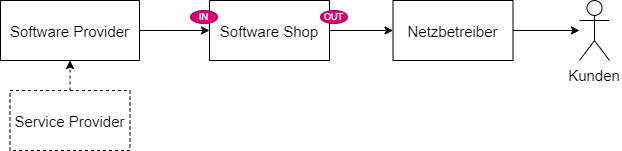
\includegraphics[width=0.9\columnwidth]{pictures/konzept-supplychain.png}
	\label{img:supplychain}
	\caption{Supply Chain von Software}
\end{figure}\\
Nach Porter ist die Wertschöpfungskette in primäre und unterstützende Aktivitäten aufzuteilen.\cite{wsk}Primäre Aktivitäten "liefern dabei einen direkten wertschöpfenden Beitrag zur Erstellung eines Produktes."\cite[Vgl.]{wsk} Unterstützende Aktivitäten sind als "notwendige Voraussetzung zu Erstellung der Produkte"\cite[Vgl. ebd.]{wsk}zu sehen. Sie sind im Rahmen aller Primäraktivitäten aktiv und beeinflussen die Qualität des Produktes. \cite{wsk2}. In Abbildung \hyperref[img:wsk]{8} werden die identifizierten Bausteine den Aktivitäten einer Wertschöpfungskette zugeordnet. Die in Kapitel \ref{key_activities} festgelegte Gruppierung der Schlüsselaktivitäten wird beibehalten und farblich hervorgehoben.

\subsubsection{Primäre Aktivitäten}
Es gibt fünf primäre Aktivitäten. Die erste Aktivität ist die Beschaffung und Lagerung von Materialien, in diesem Fall von Softwares, welche als \textbf{Eingangslogistik} bezeichnet wird. Im Kontext dieser sind zwei wichtige Bausteine zu erwähnen:
\begin{itemize}
	\item[] \hspace{-0.6cm}\textbf{Software-Sicherheit verifizieren}\\ \label{security}
	Sämtliche Softwares die dem Shop hinzugefügt werden sollen, müssen zunächst diverse Sicherheitschecks überstehen. Zum einen sollten Softwares hinsichtlich aufgenommener und gespeicherter Daten überprüft werden. Je nach Land gelten unterschiedliche Datenschutzrichtlinien, welche zu beachten sind um die Privatsphäre von Fahrzeughaltern zu schützen. Weiterhin muss festgestellt werden, dass durch die neue Software keine Sicherheitslücken bei der Fahraufgabe entstehen. Möglicherweise kann dies durch die Nutzung von Simulationen erreicht werden. \\
	Es ist sinnvoll, ein Sicherheitskonzept zu entwickeln welches die Überprüfung von Software unterstützt. Das Ziel des Sicherheitsverifikation ist letzten Endes, dass durch neues Softwares keine Gefahren für die Fahrzeuginsassen entstehen. 
	
	\item[] \hspace{-0.6cm} \textbf{Klassifizierung von Software}\\
	Erfüllt eine Software die Sicherheitsrichtlinen, wird sie anschließend Klassifiziert. Die Klassifizierung von Software soll die Suche und Darstellung dieser im Shop unterstützen, in dem der Software diverse Meta-Daten hinzugefügt werden. Teilweise können diese Meta-Daten im Shop als Such-Filter verwendet werden, einzelne geben auch an wie gut/schlecht eine Software ist und welche Aufgabe sie erfüllt. Ein beispielhaftes Konzept  wird in Kapitel \ref{sw_klassifizierung} erarbeitet und erklärt.
\end{itemize}
\begin{figure}[!h]
	\hspace{-2.5cm}
	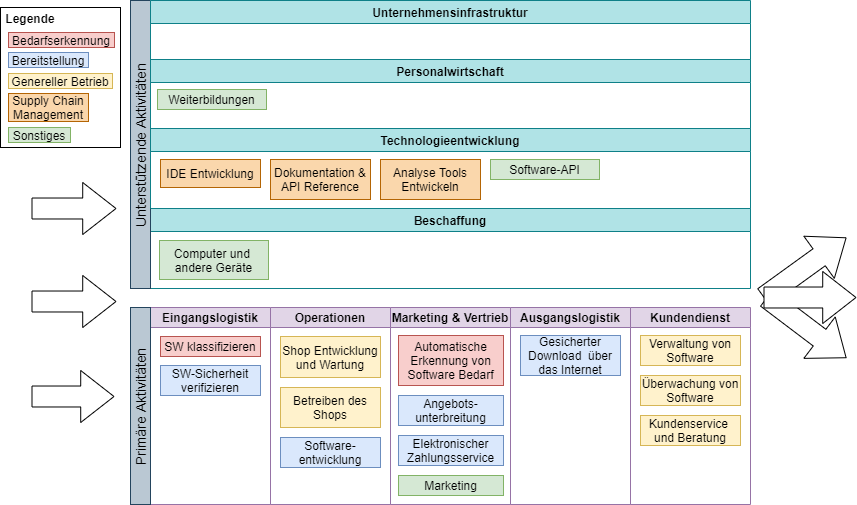
\includegraphics[width=1.2\columnwidth]{pictures/konzept-wsk.png}
	\label{img:wsk}
	\caption{Die wichtigsten Bausteine einzelner Aktivitäten der Wertschöpfungskette}
\end{figure}
Nach erfolgreichen Durchlaufen der Eingangslogistik folgen die Aktivitäten der \textbf{Operation}. Im Rahmen dieser werden die verifizierten und klassifizierten Softwares dem Shop hinzugefügt und verwaltet. Die Operationen sind die Aufgaben des Unternehmens, die den eigentlichen Mehrwert für die Kunden schaffen. 
\begin{itemize}
	\item[] \hspace{-0.6cm} \textbf{Shop (Weiter-)Entwicklung und Wartung}\\
	Der Software Shop ist das Herz des Unternehmens, ohne welchen dessen Existenz nicht möglich ist. Die (Weiter-)Entwicklung und Wartung des Shops ist daher eine der Kernaufgaben des Unternehmens. Neue Funktionen betreffen entweder das Front-End oder das Back-End des Shop. Das Front-End ist die grafische Oberfläche, die letzten Endes von den Fahrzeughaltern bedient wird. Bei der Front-End-Entwicklung kann die Verwendung des User-Centered-Designs zu einer Verbesserung von UI und UX \textit{(User-Experience)} führen. Das Back-End ist für den Fahrzeughalter nicht sichtbar. Es \textbf{verarbeitet Kauf- und Suchanfragen von Software} und muss dementsprechend schnell und effizient sein, um eine große Menge derartiger Anfragen verarbeiten zu können. Da der Shop viel Software umfasst, die von Software Providern zur Verfügung gestellt wurde, sollte bei der (Weiter-)Entwicklung des Shops auf Kritik, Verbesserungsvorschläge und Wünsche dieser eingegangen werden. Auch die übrige \textit{Community} (OEMs, Fahrzeughalter, Flottenbetreiber) sollte in die (Weiter-)Entwicklung des Shops einbezogen werden.\\
	Neben der (Weiter-)Entwicklung des Shops, muss auch die bereits existierende Plattform gewartet werden. Dies umfasst den Austausch von unzuverlässiger Hardware, aber auch das schnelle beheben von Bugs, die im Shop aufgetreten sind und die kontinuierliche Überwachung der Datenbanken, Server etc.

	\item[] \hspace{-0.6cm}\textbf{Betreiben des Shops}\\	
	Damit der Shop betrieben werden kann, muss der Inhalt dessen verwaltet werden.
	
	Softwares, die durch die Eingangslogistik klassifiziert und verifiziert wurden, müssen dem Shop hinzugefügt oder aus diesem entfernt werden und eingehende Download-Anfragen müssen verarbeitet werden. Softwares die vermehrt von Fahrzeughaltern gemeldet wurden, müssen überprüft und gegebenenfalls aus dem Shop entfernt werden. Dies kann der Fall sein, wenn eine Software Sicherheitslücken aufweist. Damit im Shop keine Inhalte \textit{(Softwares, Bewertungen von Softwares)} vorkommen, die diskriminierend, rassistische oder auf eine andere Art \& Weise Menschenrechts-verletzend sind, werden diese sofort aus dem Shop entfernt.\\
	Softwares die im Laufe der Zeit als "besonders gut" aufgefallen sind, können ein Siegel "Empfehlung der Redaktion" erhalten. Durch dieses Siegel soll die Qualität einer Software betont werden, wodurch Fahrzeughalter zum Kauf bewegt werden können. 
			
	\item[] \hspace{-0.6cm} \textbf{Eigene Softwareentwicklung}\\
	Neben der Bereitstellung von Software anderer Software Provider ist auch die eigene Entwicklung und Bereitstellung von Software im Shop wichtig. Einerseits stellt der Verkauf eigener Software weitere Einnahmequelle für das Unternehmen, andererseits lässt der Verkauf einer guten, günstigen Software die Reputation des Shops steigen. 
\end{itemize}
Die vorangegangenen Aufgaben stellen Voraussetzungen dar, welche für den Verkauf von Software notwendig sind. Der Shop ist zunächst auf Fahrzeugen installiert, aber Fahrzeughalter müssen noch zum Kauf bewegt werden. Dies passiert im dritten Teil der Wertschöpfungskette, dem \textbf{Marketing und Vertrieb} (von Software).
\begin{itemize}
	\item[] \hspace{-0.6cm} \textbf{Automatische Erkennung von Softwarebedarf}\\
	Um Fahrzeughalter beim Kauf von Software zu unterstützen soll sichergestellt werden, dass die gekauften Softwares auch tatsächlich benötigt werden. Hierzu soll der Softwarebedarf eines Fahrzeug automatisch anhand von Fahrzeugdaten identifiziert und dem Fahrzeughalter vorgeschlagen werden. Es gibt diverse Möglichkeiten den Softwarebedarf eines Fahrzeugs automatisch zu bestimmen:\\	
	\subitem \textbf{Suche anhand einer einzelnen Situation} \\
		Diese Suche wird in Kapitel \ref{2.3} beschrieben. Das Ergebnis der Suche entählt entweder \textbf{keine} oder genau \textbf{eine }Software. Die Suche soll automatisch erfolgen und die Vorschläge werden im Shop aufgezeigt.
		
	\subitem \textbf{Routen-Basierte Suche nach Software}\\
		Ebenfalls in Kapitel \ref{2.3} beschrieben, erfolgt diese Suche vor Fahrtantritt und wird im übrigen ausgeführt, wenn das Fahrzeug kurz davor ist eine nicht häufig zurückgelegte Strecke zu Fahren. Die Ergebnisse der Suche werden in die Routenplanung integriert und dem Fahrzeughalter wie in Kapitel \ref{2.3} beschrieben vorgeschlagen.
		
	\subitem \textbf{Shop-Basierte Suche \textit{(Shop-Auswahl)}}\\
		Wird eine Software unabhängig von vorherigen Suchen im Shop ausgewählt, kann der Fahrer berechnen lassen, ob und wenn ja zu welchem Umfang die jeweilige Software das Fahrspektrum des Fahrzeugs erweitert. Das Ergebnis der Anfrage stellt eine gute Entscheidungsgrundlage für den Kauf der Software dar, da dem Fahrzeughalter so der tatsächliche eigene Nutzen der Software präsentiert wird.
		
	\subitem \textbf{Umgebungsbedingte Softwaresuche}\\
		Die Umgebungssuche ist eine Weiterentwicklung der in Kapitel \ref{2.3} erwähnten \textit{Suche aus Basis der Fahrtenhistorie.} Die Idee hinter der Umgebungs-Suche ist, dass dem Fahrzeughalter Softwares vorgeschlagen werden, die andere Fahrzeuge in der Region vermehrt installiert haben. Die Umgebungs-Suche wird in Kapitel \ref{umgebungssuche} nochmals im Detail erläutert.
	
	Abhängig davon, ob passende Softwares gefunden wurden oder nicht, werden sie dem Fahrzeughalter vorgeschlagen. Durch den Prozess wird nicht nur die Kundenzufriedenheit gesteigert, sondern auch mehrere Nutzenversprechen erfüllt(NV-3, NV-4, NV-5). Neben Suchalgorithmen die dem Fahrzeughalter Softwarevorschläge unterbreiten, können Service Provider einem Fahrzeug auch eine Software vorschlagen. Dies ist notwendig, wenn der Fahrzeughalter einen Service nutzen will für den eine bestimmte Software auf dem Fahrzeug installiert sein muss.

	\item[] \hspace{-0.6cm} \textbf{Angebotsunterbreitung}\\
	Wird anhand einer der zuvor aufgelisteten SUchen festgestellt, das eine bestimmte Software dem Fahrzeug hinzugefügt werden kann, muss diese dem Fahrzeughalter vorgeschlagen werden. Im Kontext der Angebotsunterbreitung wird der Zeitpunkt festgestellt, zu welchem die Software dem Fahrer vorgeschlagen wird. Ein Konzept für diese Situationserkennung wurde in Kapitel \ref{3.3} erläutert.
	
	\item[] \hspace{-0.6cm} \textbf{Bereitstellung elektronischer Zahlungsschnittstellen}\\
	Um den Kauf einer Software abschließen zu können, müssen Fahrzeughalter den Kaufpreis über eine elektronische Zahlungsschnittstelle bezahlen können. Hierzu sollten bestenfalls mehrere gängige Zahlungsschnittstellen \textit{(MasterCard, PayPal, EC-Cash o.A.)} mit dem Shop verknüpft werden, um so mehr Fahrzeughaltern den Kauf zu ermöglichen. Um weitere eigene Umsätze zu generieren, kann hier auch eine eigene Zahlungsschnittstelle hinzugefügt werden. Fahrzeughalter können zur Verwendung dieser gebracht werden, indem der Kauf mittels dieser Schnittstelle beispielsweise günstiger oder schneller ist.
	
	\item[] \hspace{-0.6cm} \textbf{Marketing}\\
	Wie im Business Model beschrieben, ist der Umfang des Marketings maßgebend für den Erfolg des Shops. Die Kampagnen sollten auf möglichst vielen Kanälen zu sehen sein und dabei möglichst viele Alters- und Kundengruppen ansprechen. Vor allem die Vermarktung über Social Media Kanäle ist ratsam, da über diese vorwiegend junge Menschen erreicht werden. Es kann Sinnvoll sein "Markenbotschafter" zu finden, die Content für Social Media Plattformen entwerfen. Coca Cola hat dies beispielsweise erfolgreich mit Coke TV\footnote{\url{https://www.youtube.com/channel/UCTfwo-EWSD-8hZ7F8HG_qJg}, Aufgerufen am 14. Juni 2020} geschafft.
\end{itemize}
Damit die beworbenen und vorgeschlagenen Softwares letztendlich auch an die Fahrzeuge "ausgeliefert" werden können, muss die \textbf{Ausgangslogistik} strukturiert werden. Sie komplettiert die Logistik \textit{Eingangs- und Ausgangslogistik}) und legt fest, über welche Distributionskanäle Software verteilt wird.
\begin{itemize}
	\item[] \hspace{-0.6cm} \textbf{Gesicherter Download über das Internet}\\
	Die Bereitstellung von der bezahlten Software wird mit dem Download abgeschlossen. Dieser Download soll zum einen orts- und zeitunabhängig sein, außerdem muss die Download-Schnittstelle sicher sein. Um ersteres zu gewährleisten, sollte der Ausbau von Kommunikationsnetzwerken \textit{(bspw. 5G)} gefördert werden. Durch den Download von Software über das Internet können hohe Kosten für Fahrzeughalter entstehen. Durch eine Kooperation mit Mobilfunkanbietern können diese Kosten skalierbar gehalten werden, was fortlaufend die Kundenzufriedenheit sichern kann.
\end{itemize}
Damit die langfristige Zufriedenheit von Kunden sichergestellt werden kann, müssen auch nach dem Kauf für den Kunden wertschöpfende Aktivitäten durchgeführt werden. Diese werden dem letzten Schritt der Wertschöpfungskette, dem \textbf{Kundendienst}, zugeordnet.	
\begin{itemize}
	\item[] \hspace{-0.6cm} \textbf{Verwaltung von gekaufter Software}\\
	Damit Fahrzeughalter wissen, welche Softwares sie gekauft, geliehen oder gemietet haben soll für sie die eigenständige Verwaltung von Software im Shop möglich sein. Fahrzeughalter behalten hierdurch den Überblick über ihr Fahrzeug und können die Softwares entfernen oder hinzufügen.
	
	\item[] \hspace{-0.6cm} \textbf{Überwachung installierter Software}\\
	Um Fahrzeughaltern vor Augen zu führen, welche Softwares notwendig für das Fahrzeug sind und welche nicht, sollten diese Einblick in eine Art Überwachung der Software erhalten. Hier können grundlegende Statistiken geführt werden wie
	\begin{itemize}
		\item die durchschnittliche Nutzungsdauer der Software in Prozent
		\item das Datum, an welchem die Software das letzte mal genutzt wurde
		\item oder eine Liste, in welcher zu sehen ist welche Softwares an welchem Tag der Woche vermehrt genutzt werden.
	\end{itemize}
	Aufgrund der steigenden Bedeutung des Datenschutzes könnte auch eine Ansicht erstellt werden, welche zeigt welche Daten von Softwares erhoben werden. Hierdurch könnte das Vertrauen von Kunden gestärkt werden \textit{(Oder auch nicht, je nach dem welche und wie viele Daten erhoben und gespeichert werden)}.
	
	\item[] \hspace{-0.6cm} \textbf{Kundenservice und Beratung}\\
	Um vor allem die Bindung zu älteren Kunden aufzubauen, kann das einrichten einer Telefonischen Beratung für sinnvoll sein. Vor allem bei der Ersteinrichtung eines Fahrzeugs können Fahrzeughalter unterstützt werden, indem sie telefonisch beraten werden. Auch alternative, vorwiegend digitale Varianten Fahrzeughalter bezüglich Sofwtares zu beraten kann einen Mehrwert für diese bieten. Durch das entwickeln von Nutzerforen oder der Möglichkeit, Softwares zu bewerten \textit{(1-5 Sterne + Kommentar)} können Fahrzeughalter sich gegenseitig bezüglich Softwares beraten.
\end{itemize}
\textbf{Überblick}\\
Die fünf Aktivitäten der Wertschöpfungskette schaffen Mehrwerte für Fahrzeughalter. Wird eine Software von einem Software Providern beim Softwareshop "eingereicht", wird sie für den Verkauf an Fahrzeughalter vorbereitet. Jeder einzelne Schritt der Wertschöpfungskette trägt dazu bei, das Fahrzeughalter am ende selbstständig genau die Software installieren können, die sie benötigen und dabei zufrieden mit dem Ergebnis sind. Während all diese Schritte durchlaufen werden, fügen die \textit{unterstützenden Aktivitäten} stetig Mehrwerte zur Wertschöpfung hinzu und sind daher\textit{indirekt am Erfolg beteiligt}. Im folgenden diese vorgestellt und ihre Rolle im Ablauf der Wertschöpfungskette verdeutlicht.

\subsubsection{Unterstützende Aktivitäten}\label{unterstd_activities}
Es gibt vier Unterstützende Aktivitäten. Angefangen bei der Schaffung einer gut aufgebauten \textbf{Unternehmensinfrastruktur}, kann diese Alltägliche Problematiken beheben und zeit sparen. Zu dieser gehört ein gute Anbindung zur Außenwelt, schnelles Internet und Mitarbeiter freundliche Büroräume, in welchen auch Freizeitaktivitäten möglich sind. Neben der Schaffung einer guten Unternehmensinfrastruktur hat auch die \textbf{Personalwirtschaft} \textit{(Human-Resource-Management)} einen starken Einfluss auf den Erfolg des Unternehmens. Die Personalwirtschaft beschreibt wichtige, die Mitarbeiter unterstützende Strukturen und Regelungen des Unternehmens.
\begin{itemize}
	\item[] \hspace{-0.6cm} \textbf{Weiterbildungen}\\
	Die kontinuierliche Weiterbildung der Mitarbeiter ist für den Erfolg des Shops überaus wichtig. Weiterbildungen müssen nicht Zwangsweise in dem jeweiligen Fachbereich des Mitarbeiters liegen, sondern können auch neue Aspekte beleuchten. So können Entwickler einerseits gemeinsamen neue Programmiersprachen \& -frameworks lernen, anderseits können auch andere "Skills" beigebracht oder Aktivitäten \textit{(bspw. Sport)} miteinander durchgeführt werden, welche die Team-Chemie steigern. Die Schaffung einer guten Work-Life-Balance kann die Produktivität der Mitarbeiter erhöhen\cite{wlb} und somit auch den Erfolg des Shops nachhaltig sichern.
	
\end{itemize}
Für ein digitales Unternehmen ist die stetige \textbf{Technologieentwicklung} wichtig und kann wegweisend für den Erfolg des Unternehmens sein. Zu dieser gehört nicht nur die Schaffung von Werten für die innerbetriebliche Wertschöpfungskette, sondern auch die Supply Chain übergreifend Unterstützung der Partner und Kunden.

\begin{itemize}
	\item[] \hspace{-0.6cm} \textbf{IDE Entwicklung}\\
	Damit Software Provider bei der Entwicklung von Softwares unterstützt werden, ist die Bereitstellung einer eigens entwickelten Entwicklungsumgebung\textit{(IDE)} sinnvoll. 
	Diese IDE kann Features und Tools umfassen, welche explizit für die Entwicklung von (Fahrzeug-) Softwares entwickelt wurden. Durch integrierte Simulatoren und Sicherheitschecks könnte der Weg von Idee über Entwicklung hinzu Bereitstellung im Shop verkürzt werden. Ein Vergleich aus der Realität ist Android Studio\footnote{https://developer.android.com/studio} aber auch die Eclipse IDE, welche in Zusammenarbeit mit Unternehmen aus der ganzen Welt entwickelt wird.\footnote{\url{https://www.eclipse.org/org/}, Aufgerufen am \today}
	
	\item[] \hspace{-0.6cm} \textbf{Dokumentation und API-Reference}\\
	Die Entwicklung von Software wird zusätzlich durch die Bereitstellung einer ausführlichen API-Reference sowie technischen Dokumentation (mit Beispielen) positiv unterstützt. Die API-Reference sollte alle Funktionen von Klassen ausführlich beschreiben und im Nutzungskontext vorgestellt werden. Diagramme unterstützen zusätzlich das Verständnis der API. Um die Entwicklung neuer Softwares voranzutreiben ist es sinnvoll eine Einführung \textit{('Getting Started Guide')} in die Entwicklung von Softwares für ein Fahrzeug bereitzustellen. Google stellt in diesem Kontext das \textit{Android Jetpack}\footnote{\url{https://developer.android.com/jetpack}, Aufgerufen am \today} sowie weitere Dokumentationen mit Anleitungen und Videos zur Verfügung.\footnote{\url{https://developer.android.com/guide}, Aufgerufen am \today}. Auch und vor allem sollten hier die Sicherheitskriterien welche im Kontext der Wertschöpfungskette in Abschnitt \textbf{Eingangslogistik} erwähnt wurden vorgestellt werden. 
	
	\item[] \hspace{-0.6cm} \textbf{Entwicklung von Analyse-Tools}\\
	Um Software Provider zusätzlich bei der (Weiter-)Entwicklung zu unterstützen, können Analyse-Tools entwickelt werden. Anhand dieser können Statistiken von Softwares erhoben werden, durch welche Entwicklern Ideen zur Verbesserung ihrer Software leichter finden können. Dies Statistiken können generelle Kennzahlen\textit{(Nutzung in H je Tag)} aber auch spezifischere Werte \textit{(Button-Clicks)} sein, durch welche Entwickler dazu in der Lage sind, ihre Software zu verbessern.
	
	\item[] \hspace{-0.6cm} \textbf{API-Entwicklung}\\
	Damit Software Provider bestimmte Systeme von Fahrzeugen ansteuern können, müssen APIs für die jeweiligen Systeme des Fahrzeugs entwickelt werden. Über diese können Daten der Systeme ausgelesen oder eingefügt werden. Da künftig hergestellte Fahrzeuge neuartige Technologien enthalten werden, die heutzutage noch nicht existieren, müssen die APIs im Laufe der Zeit immer weiter angepasst bzw. erweitert werden.\\
	Damit "alte" Fahrzeuge weiterhin von einer Software gesteuert werden können, müssen die alten APIs aber bestehen bleiben. In Android wird diese Problematik sinnvoll durch das \textit{"API-Level"} gelöst: Jede Android Version hat ein eigenes \textit{API-Level}. Je höher das Level, desto höher auch die Android Version. Ein Smartphone mit API-Level 23 \textit{(Android 6.0)} kann alle Funktionen und Methoden \textit{"tieferer"} APIs nutzen, nicht aber die \textit{"höherer"} APIs \textit{(>23)}. Jede App hat eine \textit{minimale API-Version} welche festlegt, welches API-Level das Endgerät mindestens haben muss. Im Kontext von Fahrzeugen ist es vorstellbar, dass jedes Teilsystem eines Fahrzeugs ein eigenes mininmales API-Level hat. Softwares dadurch nur auf Fahrzeugen installiert werden, welche den Anforderungen der Software entsprechen. 
\end{itemize}

Die letzte unterstützende Aktivität ist die \textbf{Beschaffung}. Ihre Aufgabe ist, dass alle Mitarbeiter mit den nötigen Materialien, das heißt Computern, Tastaturen, Stiften oder anderem versorgt werden.\\\\
\subsection{Zusammenfassung}
Das in Kapitel \ref{bmc} erstellte Geschäftsmodell bietet einen guten Überblick das Software Shops und die damit einhergehenden Aufgaben, Kosten, Partner und Strukturen der Unternehmung. Anhand der bestimmten Kundensegmente konnten Kundenbeziehungen definiert und Aspekte des Marketings identifiziert werden. Weiterhin wurden Nutzenversprechen aufgestellt, anhand welcher die Schlüsselressourcen, -aktivitäten und -partner identifiziert wurden.\\

In Kapitel \ref{wsk} wurden die zuvor im Geschäftsmodell identifizierten Schlüsselaktivitäten sortiert und den einzelnen Aktivitäten einer Wertschöpfungskette nach Porter zugeordnet. Durch die weitere Aufteilung der Bausteine in fünf Gruppen \textit{(Bedarfserkennung, Bereitstellung, Kundenzufriedenheit, Supply Chain Management, Sonstiges)} konnte verdeutlicht werden, welchen Sinn einzelne Bausteinen haben steckt und worauf diese Einfluss nehmen.\\

Um den Ablauf eines Softwareeinkaufs im Prototypen darzustellen, werden im folgenden technische Konzepte vorgestellt die in diesem implementiert werden können.
\clearpage
\section{Technische Konzepte}\label{technische_konzepte}
Im vorherigen Kapitel wurden viele mögliche Aufgaben benannt, die im Kontext eines Software Shops entstehen können. Da in dieser Bachelorarbeit nicht alle identifizierten Bausteine im Detail diskutiert werden können, sollen die folgenden technischen Konzepte zumindest einige dieser erweitern. Im kommenden Kapitel wird ein mögliches Konzept für die Klassifizierung von Software vorgestellt, welche in der Eingangslogistik stattfindet. In Kapitel \ref{umgebungssuche} wird ein Such-Algorithmus skizziert, welcher für die automatische Erkennung von Softwarebedarf genutzt werden kann. Im letzten Kapitel werden drei Kommunikationskonzepte vorgestellt, welche den Ablauf der Kommunikation zwischen dem Fahrzeug, dem Server und den anderen Akteuren der Umwelt im Kontext bestimmter Anwendungsfälle skizzieren.
\subsection{Klassifizierung von Software}\label{sw_klassifizierung}
Das Ziel der Software Klassifikation ist es, den Fahrzeughaltern beim Kauf unterstützende Kennzahlen zur Verfügung zu stellen, anhand welcher sie sinnvollere Kaufentscheidungen treffen können und somit potentiell einen größeren Wert von der gekauften Software erhalten.

\subsubsection{Berechtigungen}
Eine dieser Kennzahlen ist die Anzahl genutzter Berechtigungen des Fahrzeugs. Nicht nur die Anzahl, sondern auch der Umfang einer Berechtigung können Kunden vom Kauf abschrecken.\footnote{quelle: android buch(1)} Eine Berechtigung erteilt einer Software die Erlaubnis, auf einzelne Systeme des Fahrzeugs zugreifen zu dürfen. Berechtigungen werden von Entwicklern zu einer Software hinzugefügt, wodurch diese im Shop für Fahrzeughalter zu sehen sind. Der Fahrzeughalter muss den Berechtigungen beim Kauf einer Software zustimmen, damit diese in vollem Umfang installiert und genutzt werden kann. Stimmen Fahrzeughalter Berechtigungen nicht zu, kann die entsprechende Software nicht gekauft werden. Durch die Verwendung von Berechtigungen kann die Sicherheit von Softwares gesteigert werden da sie verhindern, dass eine Software ohne weiteres auf alle Systeme des Fahrzeugs zugreifen kann. Im Kontext autonomer Fahrzeuge können mögliche Berechtigungen von der Architektur dieser abgeleitet werden, welche in Abbildung \hyperref[img:av_architecture]{9} dargestellt wird. 
\begin{figure}[H]
	\centering
	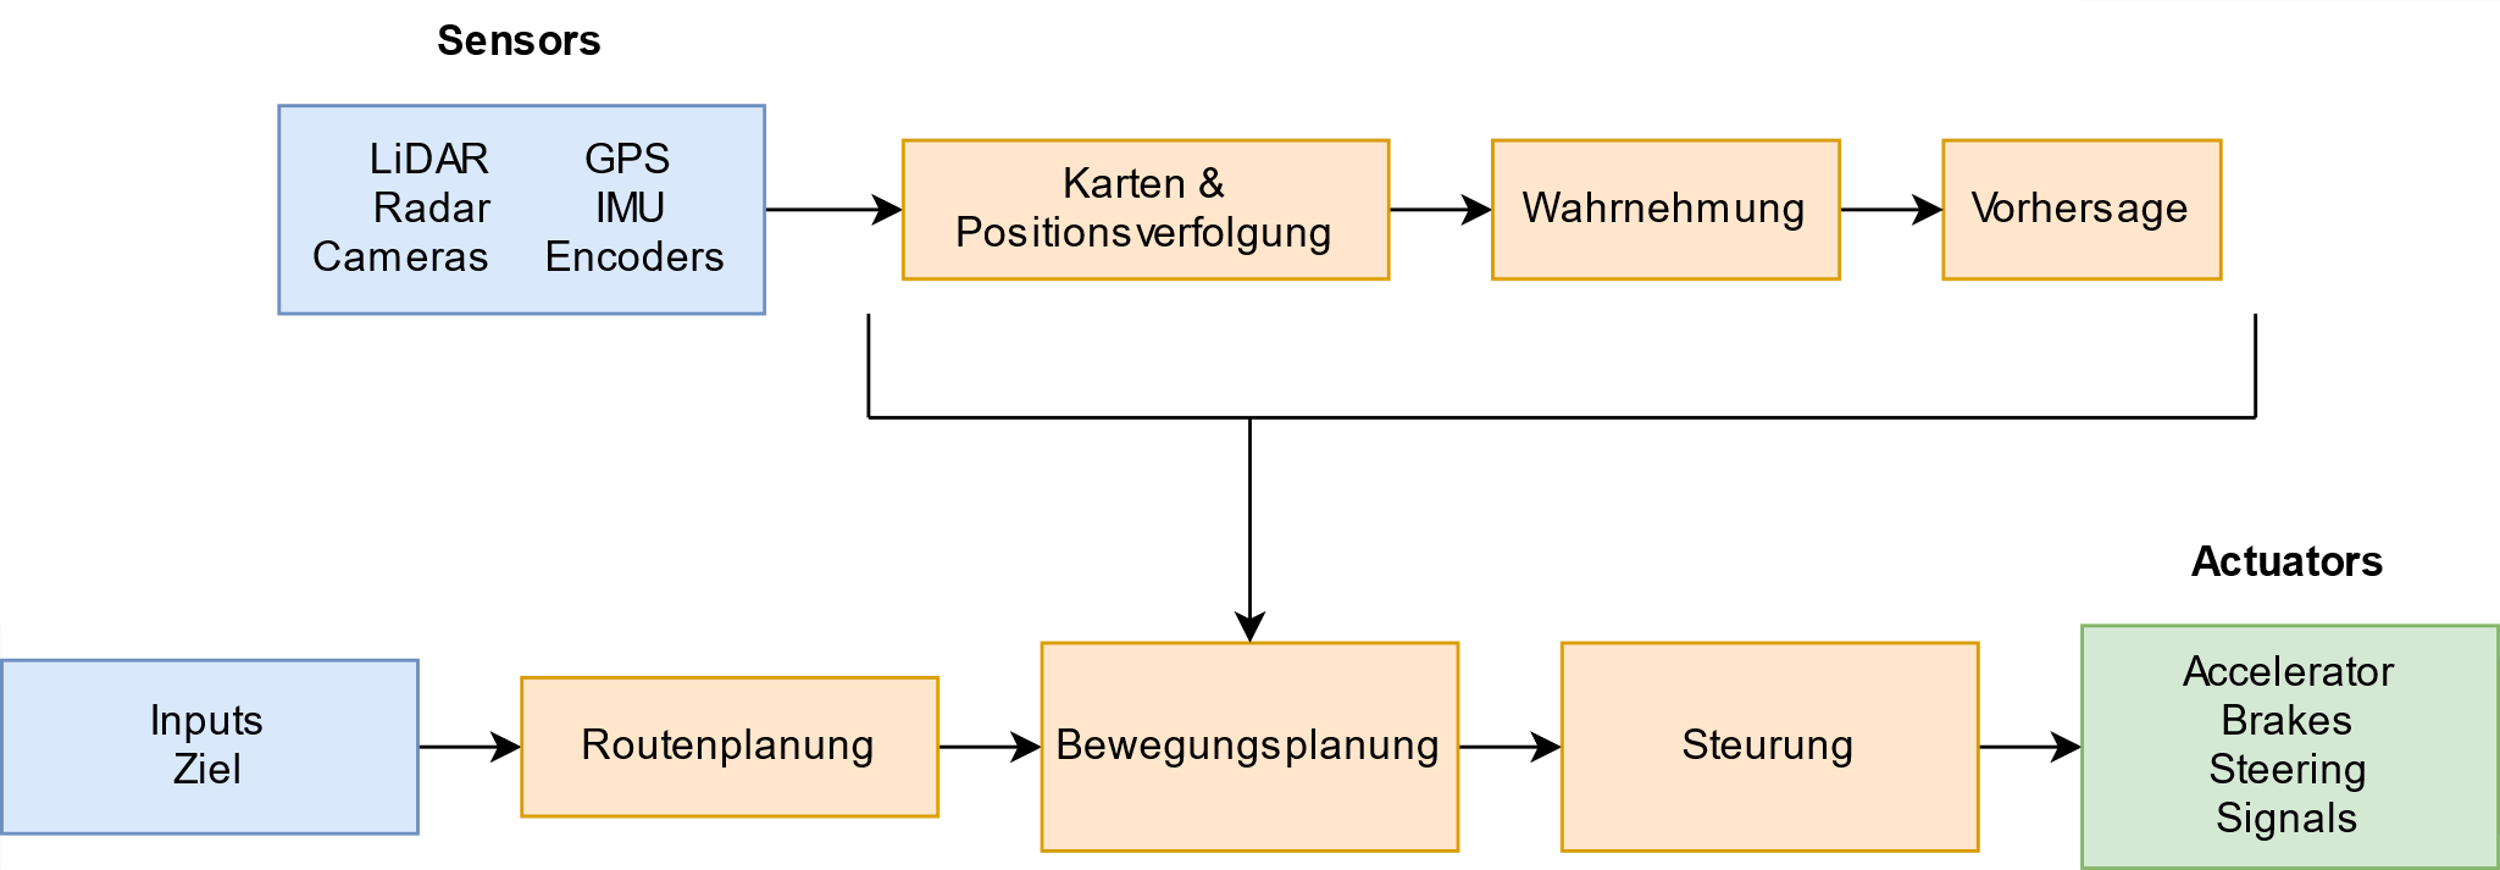
\includegraphics[width=0.95\columnwidth]{pictures/arichtecture_AV.png}
	\label{img:av_architecture}
	\caption{Jeff Schneider: Architecture of Autonomous Vehicles}
\end{figure}

Damit Berechtigungen die Fahrzeughalter davor schützen, persönliche Informationen unfreiwillig zu teilen und einer Software zu viel "Macht" über das Fahrzeug zu geben, sollte der Umfang von Berechtigungen möglichst klein gehalten werden. So sollte jede Sensorgruppe des Fahrzeugs eigene Berechtigungen haben, da die Art der aufgenommenen Informationen sich voneinander unterscheidet. So kann durch das auslesen des GPS-Sensors kontinuierlich die Position des Fahrzeugs aufgezeichnet werden, während dies über den Radar nicht möglich ist. Würde alle Sensoren über die gleiche Berechtigung zugänglich sein, würde dies eine Sicherheitslücke darstellen.\\

Neben der Privatsphäre der Fahrzeughalter ist vor allem die Sicherheit von Fahrzeuginsassen wichtig. Wird eine Software entwickelt, welche die Wahrnehmung, Vorhersage, Zieleingabe, Routenplanung, Bewegungsplanung, die Steuerung oder einzelne Aktuatoren beeinflusst, kann dies die Sicherheit der Insassen gefährden. Softwares, die diese Systeme nur auslesen aber nicht direkt beeinflussen haben keine Auswirkung auf die Fahrsicherheit. Daher sollte jedes System jeweils zwei einzelne Berechtigungen haben. Durch die eine kann ein System ausgelesen werden. Durch die andere können Systeme beeinflusst werden, wodurch aktiv in die Fahraufgabe eingegriffen wird.\\

Neben Berechtigungen, die einzelne Systeme eines Fahrzeugs benötigen, sollten auch weitere Services des Fahrzeugs nur durch die Nutzung von Berechtigungen möglich sein. Eine Berechtigung für die Nutzung des Internets ist sinnvoll, da Softwares hierdurch nicht wahllos Nutzerdaten speichern können oder sonstige Verletzungen von Datenschutz- oder sonstigen Sicherheitsrichtlinien begehen können. Auch die Kommunikation mit anderen Akteuren des Straßenverkehrs sollte über eine Berechtigung beschränkt werden.

\subsubsection{Abgeleitete Kennzahlen}
Neben der Art und Anzahl genutzter Berechtigungen einer Software, können auch andere Kennzahlen einer Software den Fahrzeughalter bei der Kaufentscheidung unterstützen. Einige dieser Kennzahlen können von den im Businessmodel beschriebenen Nutzenversprechen abgleitet werden \textit{(Kapitel \ref{nv})}.\\

Um darzustellen, dass die Lebenszeit das Autos verlängert wird \textit{(NV-4)} kann ein Wert berechnet werden, der aussagt wie gut eine Software die einzelnen Autoteile \textit{(Motor, Gertiebe, Reifen etc.)} schont. Die Berechnung dieses Werts kann in Carla erfolgen.zunächst müssen zwei Fahrzeuge simuliert werden, von denen das eine die jeweilige Software installiert hat und das andere nicht. Beide Fahrzeuge sollen die Szenarien, welche der Software beigefügt wurden, durchfahren und dabei bestimmte Werte wie die Reifenreibung, die Dämpfungsrate oder andere messen. Durch einen Vergleich der gemessenen Werte kann prozentual angegeben werden, wie stark eine Software bestimmte teile des Fahrzeugs schont \textbf{oder auch eben nicht}. Um Fahrzeughaltern vor Augen zu führen wie viel Zeit durch eine Software gewonnen werden kann \textit{(NV-6)}, sollte ein Zeitwert berechnet werden, welcher die durchschnittlich autonom zurückgelegte Zeit einer Software bestimmt. Die Berechnung sollte auf Basis realer Nutzungsdaten durchgeführt werden. Neben der durchschnittlich autonom zurückgelegten Zeit einer Software kann auch die Anzahl an Interaktionen mit der Autoumwelt ein ausschlaggebender Faktor für den Kauf einer Software sein. \\
Angenommen eine Software soll das Fahren in der Innenstadt ermöglichen. Wohnt der Fahrzeughalter nicht im Umkreis einer Stadt, würde ihm die Software nichts sonderlich viel bringen. Durch die hohe Anzahl gesparter Stunden ist der Fahrzeughalter überzeugt und kauft sich diese dennoch. Um derartige Fälle zu verhindern, sollt die Berechnungen von Kennzahlen an die jeweilige Region des Fahrzeugs angepasst sein. Weiter Kennzahlen können sein:
\begin{itemize}
	\item[\textbf{1.}]\textbf{Anzahl an Downloads und Deinstallationen}
	\item[\textbf{2.}]\textbf{Benötigter Speicherplatz der Softwrae}
	\item[\textbf{3.}]\textbf{Bewertung der Software durch Fahrzeughalter}
\end{itemize}


Die vorgestellten Softwareberechtigungen und -kennzahlen werden im Shop zu jeder Software angezeigt, wodurch Fahrzeughalter einen ersten Eindruck einer Software erhalten können. Neben der Darstellung im Shop können Kennzahlen und Berechtigungen auch als Such-Filter im Shop verwendet werden. Hierdurch wird die Suche nach bestimmter Software im Shop erleichtert und Fahrzeughalter können leichter eine für sie passende Software entdecken. 

\subsection{Umgebungsbedingte Softwaresuche}\label{umgebungssuche}
In Kapitel \ref{wsk} wurden mehrere Möglichkeiten aufgezählt, mit denen der Softwarebedarf eines Fahrzeugs automatisch bestimmt werden kann. Die im folgenden vorgestellte Umgebungssuche soll einem Fahrzeughalter Softwares vorschlagen, welche in der Umgebung des Fahrzeugs des öfteren von anderen Verkehrsteilnehmern gekauft oder genutzt wurden.\\\\
Die Umgebungssuche beginnt mit dem Verschicken einer Nachricht vom Fahrzeug an den Server. In dieser Nachricht ist das Manifest des Fahrzeugs enthalten, auf welchem unter anderem eine Liste aller installierter Softwares eines Fahrzeugs zu finden ist. Außerdem werden Fahrdaten  verschickt, anhand welcher eine "Heatmap" erstellt werden kann durch welche ersichtlich wird, in welchen Regionen sich das Fahrzeug zuletzt aufgehalten hat. Der Server sucht innerhalb dieser Regionen nach Softwares, die von anderen Fahrzeugen in diesen gekauft wurden und noch nicht auf dem anfragenden Fahrzeug installiert sind. Ist die Suche abgeschlossen wird geprüft, ob die gefundenen Softwares einen Mehrwert für das Fahrzeug bieten. Um dies zu bestimmen, können die einer Software beigelegten Open Scenario Dateien genutzt werden, indem diese in einer Simulation durchfahren werden.\\

Zunächst wird eine virtuelle Instanz des Fahrzeugs anhand des versendeten Manifests erstellt \textit{(Originalinstanz)}. Für jede gefundene Software wird eine weitere Instanz des Fahrzeugs erstellt, auf welcher zusätzlich die Software installiert wird\textit{(Neue Instanz)}. Nach dem erstellen der virtuellen Fahrzeuge, durchlaufen die Originalinstanz und die neue Instanz die jeweiligen Szenarien der neuen Softwares. Durch einen Vergleich der Simulationen soll festgestellt werden, ob eine Software positive, negative oder überhaupt keine Auswirkungen auf das Fahrverhalten des Fahrzeugs hat. Positiv ist, wenn das Fahrzeug die Situation nun selbstständig durchfahren kann oder dies Ressourcenschonender tut. Negativ  ist es, wenn die Situation durch die neue Software nicht weiter durchfahren wird oder die neue Software zum durchfahren der Situation nicht vom Fahrzeug ausgewählt wird. Dies kann bedeuten, dass auf dem Fahrzeug bereits eine Software installiert ist, welche diese bereits abdeckt.

\subsection{Kommunikationsprotokolle}\label{4.2}
Damit Software heruntergeladen und anschließend genutzt werden kann, müssen das Fahrzeug, der Software Shop und auch potentiell weitere Akteure des Straßenverkehr \textit{(Autos, Ampeln, Service Provider, oA.)} miteinander kommunizieren. Damit diese Kommunikation sicher und geordnet ist, werden drei Kommunikationsprotokolle erstellt die im Kapitel \ref{prototyp} implementiert werden können. Die Kommunikation zwischen dem Fahrzeug und dem Server kann durch das einbinden der Uptane-Architektur (\ref{3.1}) und einhergehender Lösungsansätze sicherer gestaltet werden. So enthält jede Nachricht die ein Fahrzeug an den Server schickt das jeweilige Manifest des Fahrzeugs, durch welches der Server das Fahrzeug verifizieren kann und diesem anschließend neue Softwares hinzufügen kann.

\subsubsection{Kommunikationsprotokoll: Selbstständiger Softwarekauf}
\begin{wrapfigure}{R}{0.5\textwidth}
	\centering
	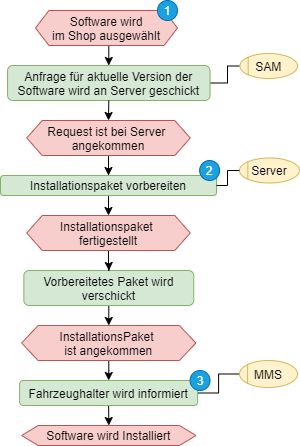
\includegraphics[width=0.48\textwidth]{pictures/konzept-Eigene-Installation.png}	\label{img:eigenstaendigIns}
	\caption{Eigenständige Installation von Software}
\end{wrapfigure}
Das in Abbildung \hyperref[img:eigenstaendigIns]{10} dargestellte Protokoll stellt den Kommunikationsablauf beim Kauf einer spezifischen Software dar. Der Fahrzeughalter kann im Shop nach Softwares suchen, indem der Name einer Software gesucht wird oder Suchfilter verwendet werden. Wurde eine Software ausgewählt \textit{(1)}, wird eine Installationsanfrage für diese an den Server geschickt. Kann die Software auf dem Fahrzeug installiert werden, bereitet der Server ein \textbf{Installationspaket} vor \textit{(2)}. In diesem ist die Software, eine neue Version des Manifests und das Angebot für die Software enthalten. Ist das Installationspaket vorbereitet, wird es an das Fahrzeug verschickt und der Fahrzeughalter wird über die Mensch Maschine Schnittstelle über darüber informiert\textit{(3)}. Abschließend wird die Software auf dem Fahrzeug installiert und der Fahrzeughalter kann sie nutzen.
\clearpage
\subsubsection{Kommunikationsprotokoll: Installationsvorschlag vom Service Provider}
In Abbildung \hyperref[img:installationsProtokollExtern]{11} wird dargestellt, wie ein Service Provider einem Fahrzeug eine Software vorschlagen kann. Die Notwendigkeit hierfür besteht, da zur Nutzen eines Services jeweils eine bestimmte Software notwendig ist. Vorzustellen sei folgende Situation: Ein Fahrzeughalter möchte in der Oldenburger Innenstadt einkaufen gehen und muss hierfür sein Fahrzeug parken. Über das Navigationssystem wählt er einen Parkplatz aus den das Fahrzeug daraufhin ansteuert. Um ein Parkticket für diesen Parkplatz kaufen und das Fahrzeug automatisch einparken zu können, benötigt dieses eine bestimmte Software. Am Parkplatz angekommen, fährt das Fahrzeug in das Sichtfeld des Parkautomaten, auch \textit{Registrierungszone} genannt \textit{(1)}. Wird ein Fahrzeug erkannt, registriert sich der Parkautomat beim Fahrzeug. Ist die Registrierung im Fahrzeug angekommen überprüft der Software Applikation Manager, ob die für den Service benötigte Software bereits auf dem Fahrzeug installiert\textit{(2)}.\\
Ist dies der Fall, wird zusätzlich überprüft ob die installierte Version der Software aktuell ist. Wenn ja, kann der Service genutzt werden - wie die Nutzung eines Service abläuft, wird im dritten und letzten Kommunikationsprotokoll dargestellt. Ist die Software noch nicht Installiert oder die installierte Version ist nicht mehr aktuell wird der Fahrzeughalter gefragt, ob er die Software Aktualisieren bzw. Kaufen möchte \textit{(4)}. Er kann das ihm vorgestellte Angebot entsprechend seiner Bedürfnisse für die Software anpassen \textit{(Leihe statt Kauf, etc.)} und seine Entscheidung durch eine Eingabe in der Mensch Maschine Schnittstelle bestätigen. Wird die Anfrage abgelehnt, wird keine Software installiert. Das Fahrzeug verlässt die Registrierungszone wieder und kann nicht auf dem Parkplatz parken. Nimmt der Fahrzeughalter die Anfrage hingegen an, sendet das Fahrzeug eine Installationsanfrage an den Server.  Der Server nimmt die Anfrage an und erstellt ein Installationspaket für die entsprechende Software \textit{(5)}. Das erstellte Paket wird an das Fahrzeug gesendet, auf diesem installiert und das Fahrzeug kann den angebotenen Park-Service nutzen. 
\begin{figure}[!h]
	\centering
	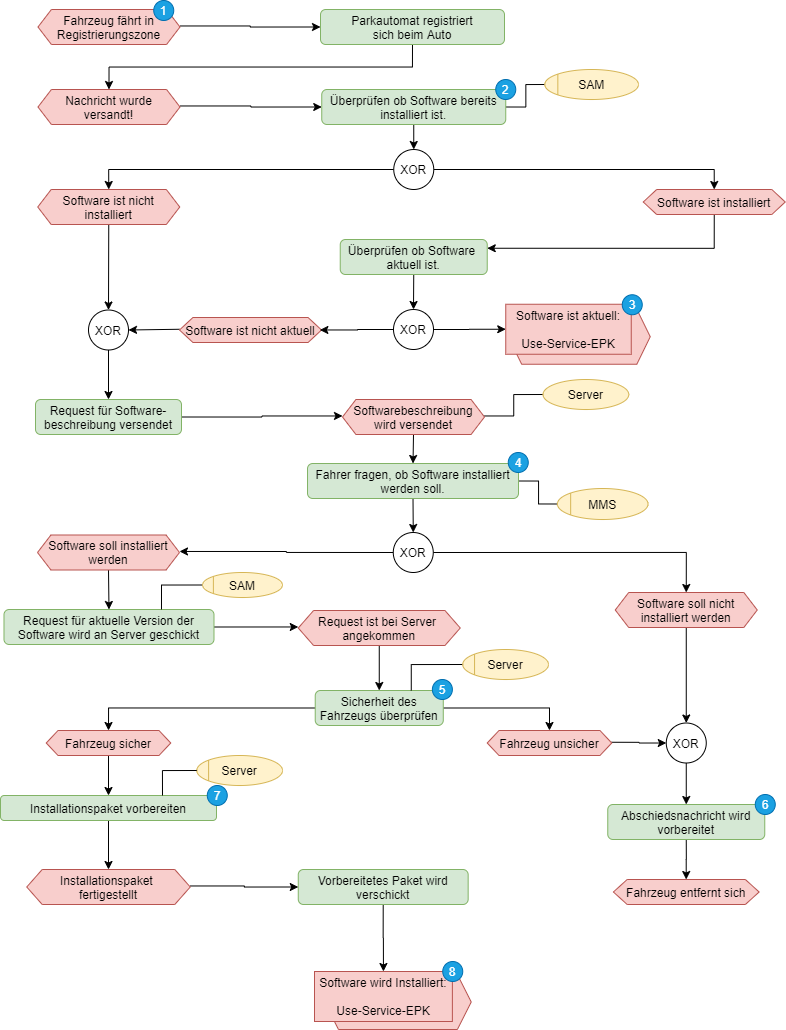
\includegraphics[width=\columnwidth]{pictures/konzept-Installationsprozess.png}
	\label{img:installationsProtokollExtern}
	\caption{Installationsprozess von Software}
\end{figure}
\subsubsection{Kommunikationsprotokoll: Nutzung eines Service}
Abbildung \hyperref[img:nutzung]{12} zeigt den Kommunikationsablauf zwischen einem Fahrzeug und einem Service Provider Actor \textit{(bspw. ein Parkautomat)}. Der dargestellte Ablauf findet statt, wenn ein Fahrzeug einen Service nutzen möchte und die aktuelle Version der hierfür notwendigen Software bereits auf dem Fahrzeug installiert ist \textit{(1)}. Der Service wird über die Mensch Maschine Schnittstelle zur Nutzung vorgeschlagen \textit{(2)} und der Fahrer kann entscheiden, ob er dies tun möchte oder nicht. Die Entscheidung des Fahrers wird an den Parkautomaten gesendet \textit{(3)}, welcher die Entscheidung evaluiert und dementsprechend dem Fahrzeug entweder einen Parkplatz zuweist oder es verabschiedet. Die jeweilige Antwort wird an das Fahrzeug gesendet und über die MMS angezeigt. Das Fahrzeug plant die kommende Bewegung und fährt dementsprechend entweder zu dem ihm zugewiesenen Parkplatz oder verlässt die Registrierungszone wieder.
\begin{figure}[!h]
	\centering
	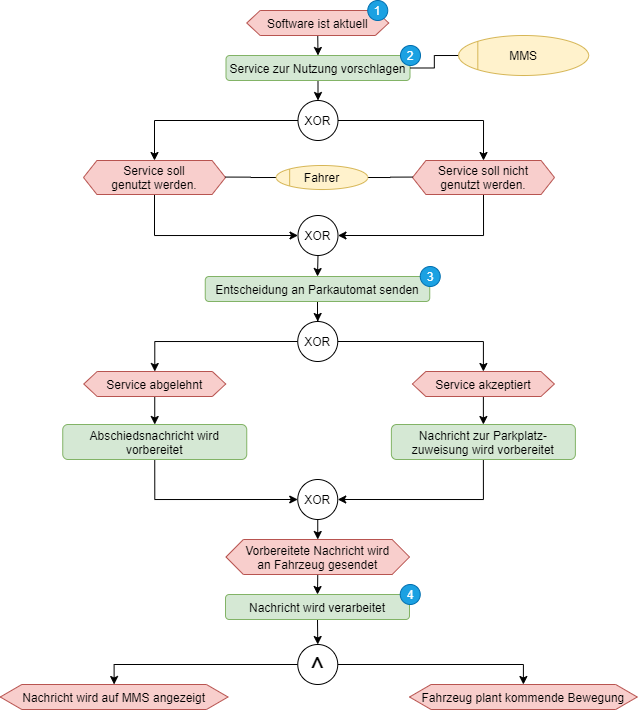
\includegraphics[width=0.8\columnwidth]{pictures/konzept-Nutzungsprozess.png}
	\caption{Nutzungsprozess von Software}
	\label{img:nutzung}
\end{figure}
\clearpage
\subsection{Ausblick}
Die in diesem Kapitel erstellten Konzepte wurden mit der Intention entwickelt, einzelne Bausteine der Wertschöpfungskette zu detaillieren und im Prototypen implementiert zu werden. Die Identifikation von Berechtigungen für einzelne Systeme eines Fahrzeugs bieten eine geeignete Grundlage, die Sicherheit intelligenter Fahrzeuge zu unterstützen. Fahrzeughalter können durch diese und weitere Kennzahlen bessere Kaufentscheidungen treffen und ihr Fahrzeug so erweitern, dass es auf deren Ansprüche angepasst ist. Die Kommunikationsprotokolle wurden erstellt, um einen Ablauf für den Prototypen aufstellen und nachverfolgen zu können. Die Kommunikationsprotokolle, die im Forschungsseminar erarbeitete Softwarearchitektur und auch weitere in der Arbeit gewonnene Erkenntnisse und Ideen werden im Prototypen eingebunden und visuell veranschaulicht.\\\\\\\\\\\\\\\\\\\\\\
\clearpage
%\section{Architektur des Prototypen}
Der entwickelte Prototyp ist ein Kernbestandteil dieser Arbeit. In diesem Kapitel werden die generelle Architektur, aufgetretene Herausforderungen und technische Details erläutert. Das Kapitel \hyperref[architecture]{4.2} umfasst eine technische Dokumentation des Prototypen.
\subsection{Anforderungen}
Die Anforderungen haben sich im Laufe der Entwicklung geändert und weiterentwickelt. Die Anforderungen sind im wesentlichen Architektur- und Codestil-Entscheidungen sowie Funktionsanforderungen.\\

\begin{center}
	\begin{tabularx}{0.9\linewidth}{|c|X|}
		\hline
		\multicolumn{2}{|l|}{\textbf{Technische Anforderungen}}\\
		\hline
		
		\textbf{\hyperref[tecreq1]{tec\_req1}} & Darstellen eines kompletten Absatzprozesses von Software.\\
		\hline
		
		\textbf{\hyperref[tecreq2]{tec\_req2}} & Verwendung von Carla für das darstellen des Autos.\\
		\hline
		
		\textbf{\hyperref[tecreq3]{tec\_req3}} & Einbeziehen von Uptane Architektur in die eigene.\\
		\hline
		
		\textbf{\hyperref[tecreq4]{tec\_req4}} & Monitoring \& Steuerung der Module.\\
		\hline
		
		\textbf{\hyperref[tecreq5]{tec\_req5}} & Verwenden von Android Automotive OS für die Mensch Maschine Schnittstelle.\\
		\hline
		
		\textbf{\hyperref[tecreq6]{tec\_req6}} & Bewahren einer erweiterbaren Architektur.\\
		\hline
		
		\textbf{\hyperref[tecreq7]{tec\_req7}} & Ordentliches JavaDoc\\
		\hline
		
	\end{tabularx}
\end{center}

\textbf{1. Darstellen eines kompletten Absatzprozesses von Software.}\label{tecreq1}\\
Im Rahmen der \hyperref[wsk]{Wertschöpfungskette} wurde ein \hyperref[absatzprozess]{Absatzprozess }für den behandelten \hyperref[anwendungsfall]{Anwendungsfall} ausgearbeitet. Die einzelnen Schritte sollen im Prototypen ausgewählt und durchgeführt werden können. Die einzelnen Schritte sollen in einer GUI angezeigt werden, der aktuelle Schritt soll farblich hervorgehoben werden. In einem Textfeld soll eine Beschreibung des aktuellen Schrittes stehen. Diese stellt dar, was welche Komponente in diesem Schritt tut.\\

\textbf{2. Verwendung von Carla für das darstellen des Autos.}\label{tecreq2}\\
Ein visuelles Durchlaufen des \hyperref[absatzprozess]{Absatzprozesses} soll das Verständnis des Anwendungsfalls steigern. Dazu müssen die Daten der Simulation ausgewertet werden, da die Position des Fahrzeugs maßgebend für den aktuellen Schritt ist.\\

\textbf{3. Einbeziehen von Uptane Architektur in die eigene.}\label{tecreq3}\\
Ein wichtiger Aspekt im Rahmen der Verteilung von Software ist das schaffen einer gesicherten Kommunikation zwischen Fahrzeug und Software-Server. Hierzu soll die im Forschungsseminar vorgestellte \hyperref[uptane]{Uptane Architektur} in die des Prototypen einfließen. Verschlüsselungen und weitere Details von Uptane werden nicht beachtet.\\

\textbf{4. Monitoring \& Steuerung des Absatzprozesses}\label{tecreq4}\\
Jedes Modul des Prototypen ist im Absatzprozess aktiv. Teilweise müssen Module während eines Schrittes auf die Antwort eines anderen Moduls warten, oder ein Modul verschickt eine Nachricht an ein anderes. Damit der Ablauf des Absatzprozesses verdeutlicht wird, sollen in einer GUI die aktuelle Status der Module abgebildet werden. Auch soll jedes Modul steuerbar sein, damit die Einzelentscheidungen des Prozesses veranschaulicht werden.\\

\textbf{5. Verwenden von Android Automotive OS für die Mensch Maschine Schnittstelle.}\label{tecreq5}\\
Über eine Android-Schnittstelle soll mit dem Auto interagiert werden. Hierzu wird eine Applikation bereitgestellt, über welche der Nutzer Entscheidungen bzgl. der Installation und Nutzung von Software eingeben kann.\\ 

\textbf{6. Bewahren einer erweiterbaren Architektur.}\label{tecreq6}\\
Sämtliche Module sollen das einbinden neuer Anwendungsfälle einfach handhaben können. Die Architekturen der Module soll dies unterstützen.\\

\textbf{7. Ordentliches JavaDoc}\label{tecreq7}\\
Damit der Code auch nach der Abgabe der Arbeit genutzt und erweitert werden kann, ist ein ordentliches JavaDoc zu führen.\\

\subsection{Technische Dokumentation}\label{architecture}
Nach \hyperref[tecreq3]{Anforderung Drei} soll die Uptane Architektur in die des Prototypen einbezogen werden. Diese wurde im Rahmen von Kapitel \hyperref[uptane]{2.2.1} vorgestellt und in ein erstes technisches Konzept \textit{(\hyperref[technGrundkonzept]{Kapitel 4})} eingearbeitet. Im folgenden wird die Architektur des Prototypen vorgestellt, welche ihren Ursprung aus dem zuvor erstellten Konzept zieht.\\
\begin{figure}[!h]
	\centering
	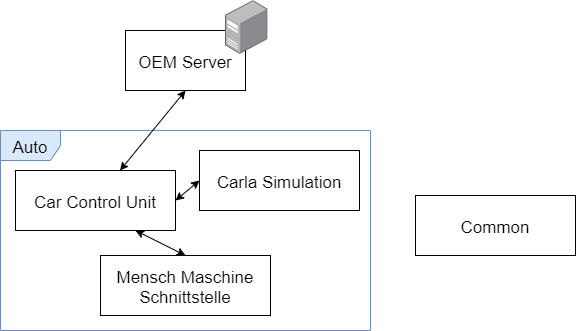
\includegraphics[width=0.8\columnwidth]{pictures/basic.png}
	\label{img:basic}
	\caption{Grundlegende Komponenten}
\end{figure}\\

Wie in Abbildung \ref{img:basic} zu sehen, umfasst der Prototyp mehrere Teilsysteme. Die Zwei wesentlichen Modulen sind der \textbf{OEM-Server} und das \textbf{Auto} \textit{(Ego-Car)}. Der OEM-Server repräsentiert die Kommunikationsinfrastruktur des Automobilherstellers und ist für das Auto die '\textbf{single source of truth}'. Das Auto wird durch die Zusammensetzung von \textbf{Mensch-Maschine-Schnittstelle} \textit{(HMI)}, \textbf{Car-Control-Unit} \textit{(CCU)} und der \textbf{Carla Simulation} dargestellt.
Die Carla Simulation beinhaltet die Darstellung eines Autos, dem 'Ego-Car', sowie der Simulation der Autoumwelt. Dieses Modul bestimmt den aktuellen Stand der Simulation, da aus der Position des Autos die möglichen Aktionen hervorgehen. Die Car-Control-Unit ist eine Kommunikations- und Steuereinheit des Autos dar und ist für die Verwaltung und Nutzung von Software zuständig. Damit eine Software auf Nutzereingaben reagieren kann, wird eine Mensch-Maschine-Schnittstelle in Form einer Android Nutzeroberfläche integriert, über welche mit dem \textbf{Auto}\textit{(blauer Kasten Abbildung \ref{img:basic})} interagiert werden kann.\\
Sämtliche Komponenten kommunizieren untereinander auf Basis der \textbf{Common Objekte}. Diese sind eine Ansammlung an Nachrichten und Objekten, welche zwischen den Komponenten verschickt werden.\\
\subsubsection{Kommunikation und Common Objekte}
\textbf{Architektur}\\
Damit die Module miteinander kommunizieren können werden Netzwerkinfrastrukturen zwischen ihnen aufgespannt \textit{(repräsentiert durch die Pfeile)}. Der OEM-Server und die CCU kommunizieren miteinander über eine Netty\footnote{QUELLE}-Verbindung. Die CCU ist mit der Carla Simulation und dem MMS jeweils über Ports verbunden. Neben diesen Netzwerkkommunikationsmethoden nutzen die Komponenten die Common-Objekten als gemeinsame Kommunikationsgrundlage. \\
\begin{figure}[!h]
	\centering
	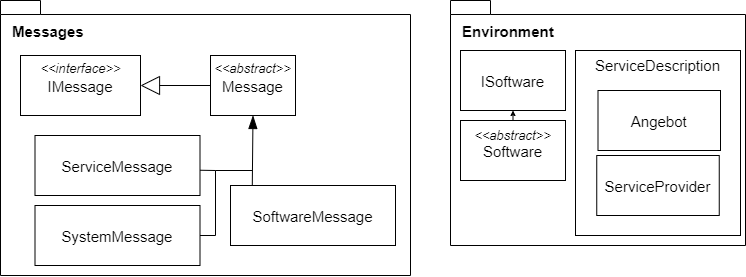
\includegraphics[width=\columnwidth]{pictures/common.png}
	\label{img:common}
	\caption{Architektur: Common Objekte}
\end{figure}\\
\textbf{Messages}\\
Das Interface \textit{IMessage} ist die oberste Klasse der Common Objekte. Sie extended java.io.Serialiable, damit die Objekte zu ByteCode umgewandelt und über die Netzwerke verschickt werden können. Die abstrakte Klasse \textit{Message }ist die Elternklasse aller folgenden Nachrichten und implementiert die Methoden \textit{IMessage}. Fort folgend wird bei allen Nachrichten zwischen \textit{Service-, Software- und SystemMessages }unterschieden. Jede dieser Klassen extended die \textit{Message}-Klasse und ist jeweils für einen wesentlichen Teil der Kommunikation zuständig.\\
\\
\textbf{Technische Dokumentation}\\
\begin{center}
	\begin{tabular}{| p{0.25\textwidth} | p{0.7\textwidth} |}
		\hline
		\textbf{Klasse} &\textbf{Beschreibung}\\
		\hline
		\textbf{ServiceMessage} &
		Jede Nachricht die im Bezug auf eine \textit{Software} verschickt wird, extended diese Klasse. In ihr wird die SoftwareID gesetzt, anhand welcher das Auto weiß auf welche Software sich die Nachricht bezieht.\\
		&
		\begin{itemize}
			\item[] \textbf{requiredSWID: String} \textit{Die ID der benötigten Software.}
			\item[] \textbf{serviceID: String} \textit{Die ID des Service Anbieters.}
		\end{itemize}\\
		\hline
		\textbf{ServiceActionMessage} \textit{extends ServiceMessage}&Die ServiceActionMessage wird von dem ServiceAnbieter\textit{(CarlaEnvironment)} an das Fahrzeug gesendet, wenn der Service genutzt werden soll. Das Fahrzeug schickt sie weiter an das CarlaCar.\\&\\
		\hline
		
	\end{tabular}
\end{center}

\textbf{Hier ist geplant:}
\begin{itemize}
	\item Jede Message beschreiben und die Assoziation zum Absatzprozess darstellen
	\item Jedes COmmonObjekt und dessen Bedeutung für den prototypen beschreiben
\end{itemize}



\subsubsection{Car-Control-Unit}
\textbf{Hier ist geplant:}
\begin{itemize}
	\item Die technische Architektur beschreiben und Lebenszyklus darstellen
	\item Bedeutung von \textbf{MessageHandler} und \textbf{SoftwareManager} verdeutlichen
	\item Auflisten: Nachrichten die von CCU verschickt bzw. empfangen werden und der Kontext der Nachrichten
	\item Herausforderungen in der implementierung
	\item ca. 4-5 Seiten
\end{itemize}

\begin{figure}[!h]
	\centering
	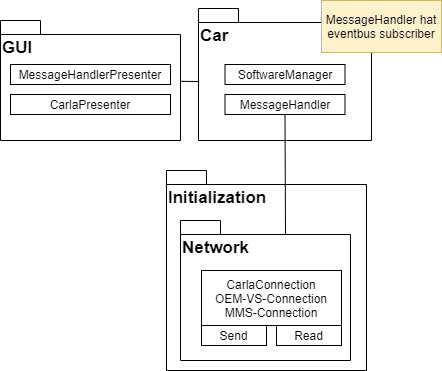
\includegraphics[width=0.8\columnwidth]{pictures/ccu.png}
	\label{img:ccu}
	\caption{Grundlegende Komponenten}
\end{figure}



\subsubsection{Software Server}\label{server}
\textbf{Hier ist geplant:}
\begin{itemize}
	\item Die technische Architektur beschreiben und Lebenszyklus darstellen
	\item Architektur im bezug auf Uptane erklären
	\item Auflisten: Nachrichten die von SwS verschickt bzw. empfangen werden und der Kontext der Nachrichten
	\item Herausforderungen in der implementierung
	\item ca. 2-3 Seiten
\end{itemize}

\begin{figure}[!h]
	\centering
	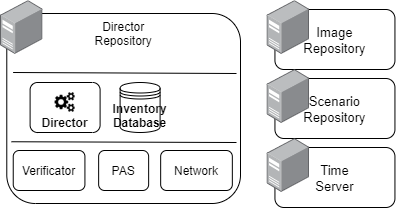
\includegraphics[width=0.8\columnwidth]{pictures/sws.png}
	\label{img:sws}
	\caption{Grundlegende Komponenten}
\end{figure}

\subsubsection{Carla}
\textbf{Hier ist geplant:}
\begin{itemize}
	\item Die technische Architektur beschreiben und Lebenszyklus darstellen
	\item Differenzieren: CarlaCar  vs. CarlaEnvironment
	\item Auflisten: Nachrichten die von Carla verschickt bzw. empfangen werden und der Kontext der Nachrichten
	\item Herausforderungen in der implementierung
	\item ca. 3-4 Seiten
\end{itemize}

\subsubsection{Mensch-Maschine-Schnittstelle}
\textbf{Hier ist geplant:}
\begin{itemize}
	\item Die technische Architektur beschreiben und Lebenszyklus darstellen
	\item Auflisten: Nachrichten die von MMS verschickt bzw. empfangen werden und der Kontext der Nachrichten
	\item ca. 2 Seiten
\end{itemize}
.
\subsection{Erweiterbarkeit und Veröffentlichung}
Dieses Kapitel kommt zum Schluss. Wird darstellen, wie der Prototyp zu erweitern ist\\
Guide: Wie füge ich eine neue SOftware + Service hinzu?
%\clearpage
\section{Vorstellung des Prototypen}\label{prototyp}
Der Prototyp demonstriert, wie eine Software entsprechend der in Kapitel \ref{bmc} identifizierten Bausteine einem Fahrzeughalter bereitgestellt werden kann. Konkret wird die Bereitstellung einer Software dargestellt, mit welcher \textbf{ein Fahrzeug selbstständig ein Parkticket kaufen und anschließend zum Parkplatz fahren kann.} Zunächst wird in Kapitel 5.1 dargestellt, wie der Prototyp installiert werden kann. Im Anschluss daran wird in Kapitel 5.2 die Software Architektur des Prototypen vorgestellt. Abschließend werden die Funktionen des Prototypen vorgestellt und wie diese genutzt werden können. 

\subsection{Architektur des Prototypen}	
Abbildung \hyperref[img:basic]{13} zeigt die Grundlegende Architektur des Prototypen. Über den OEM-Server \textit{(Server)} können Softwares Heruntergeladen werden. Der \textbf{Software Applikation Manager} \textit{(SAM)}, die \textbf{Carla Simulation} und die \textbf{Mensch Maschine Schnittstelle} \textit{(MMS)} bilden gemeinsam die Repräsentation des Fahrzeugs. Die Python-basierte Carla Simulation stellt das Fahrzeug in einer Stadt dar. Dieses Fahrzeug ist die visuelle Repräsentation des Prototypen. Dies restlichen Module sind alle in Java geschrieben. Die Mensch Maschine Schnittstelle ist eine Android-Schnittstelle, auf welcher eine Version des Software Shops als App installiert ist. Über diese App können Nachrichten von dem Software Applikation Manager empfangen und verarbeitet werden. Außerdem können Nutzereingaben getätigt werden um mit dem restlichen Kompnenten des Fahrzeugs zu kommunizieren. Der Software Applikation Manager ist mit allen Modulen des Prototypen verbunden und stellt daher die zentrale Steuerungseinheit des Prototypen dar. Außerdem erfolgt die Installation und Nutzung von Software auf diesen.
\begin{figure}[!h]
	\centering
	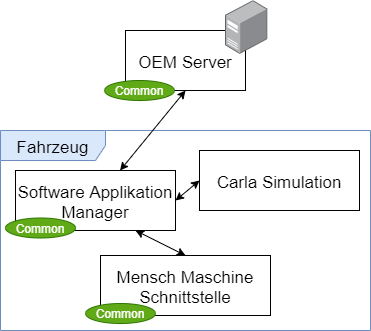
\includegraphics[width=0.5\columnwidth]{pictures/konzept-basic.png}
	\label{img:basic}
	\caption{Grundlegende Architektur der Prototypen}
\end{figure}

Der Server, SAM und die MMS kommunizieren alle auf Basis der \textbf{Common-Objekte}. Diese sind eine Sammlung an Java-Objekten, welche für die Zweckgebundene Kommunikation jedem einzelnen Modul bekannt sein muss. Sie enthalten Primitive Werte \textit{(Integer, String, Long, etc.)} und leiten alle vom Serializable-Interface ab. Abbildung \hyperref[img:common]{14} stellt die generelle Aufteilung der Objekte in zwei Gruppen dar. \\

\textbf{Environment-Objekte} sind Objekte, welche zur Umwelt des Prototypen gehören. Damit der Server spezifische Softwares verschicken kann, wird ihm die abstrakte Klasse Software zur Verfügung gestellt als auch eine Sammlung von Softwares. Jede Software des Prototypen benötigt eine eindeutige ID und eine Methode \textit{handleMessage()}, welche bestimme Messages bearbeiten kann. Auch der Software Applikation Manager nutzt diese Objekte, um so die Softwares \textit{installieren und nutzen} zu können. Die Description wird genutzt, um Softwares oder Services, die im Prototypen implementiert werden zu beschreiben. Das Provider-Objekt tut eben dies für die Beschreibung das Anbieters der Software bzw. des Services. Das Angebot repräsentiert die Auswahlmöglichkeiten, die dem Fahrzeughalter beim Kauf einer Software über die MMS vorgeschlagen werden \textit{(Kauf, Leihe, Abo)}. Alle Drei Objekte werden in der MMS genutzt um das Angebot darzustellen.

\begin{figure}[!h]
	\centering
	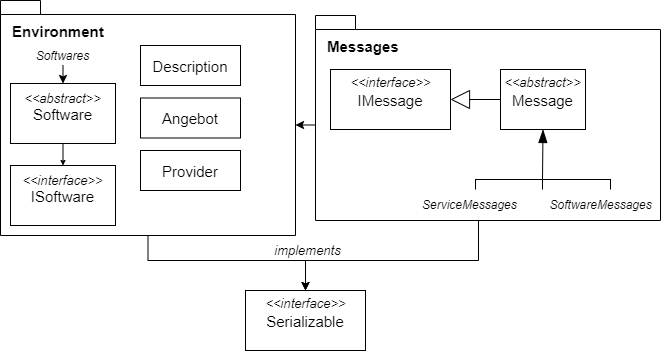
\includegraphics[width=0.8\columnwidth]{pictures/konzept-Common.png}
	\label{img:common}
	\caption{Aufbau der Common Library}
\end{figure}

Neben den Environment-Objekten gibt es auch noch Messages. Messages sind die Objekte, die im Prototypen zwischen den einzelnen Komponenten verschickt werden. Sie beinhalten neben Primitiven Datentypen auch Environment Objekte und sind ebenfalls für die zweckgebundene Kommunikation gedacht. Messages werden in SoftwareMessages oder ServiceMessages unterteilt. SoftwareMessages sind all jene Nachrichten, welche zur Installation oder Nutzung einer Software notwendig sind und ServiceMessages sind jene, die zur Nutzung eines Service notwendig sind. 

\subsubsection{Architektur des Software Applikation Managers (SAM)}
Wie zuvor erwähnt, wird über den Software Applikation Manager das Geschehen des Prototypen gesteuert. Er ist, wie in Abbildung \hyperref[img:sam]{15} zu sehen ist, in drei kleine Module aufgeteilt. In der GUI werden alle Ereignisse des Prototypen in einem Log dargestellt. Die Log-Einträge werden vom MessageHandler eingetragen. In der "Software Control Unit" baut der MessageHandler Netzwerkverbindungen zwischen sich, dem Server, der MMS und Carla auf. Jede eingehende Nachricht wird von ihm empfangen und verarbeitet. In diesem Kontext, kann eine eingegangene Nachricht an das MMS weitergeleitet werden oder es wird auf eine Nutzereingabe in der GUI gewartet. Außerdem beinhaltet der Messagehandler den SoftwareManager. Dieser verwaltet die auf dem "Fahrzeug" installierten Softwares und stellt diese zur Verfügung wenn sie zur Auswertung einer Nachricht benötigt werden.
\begin{figure}[!h]
	\centering
	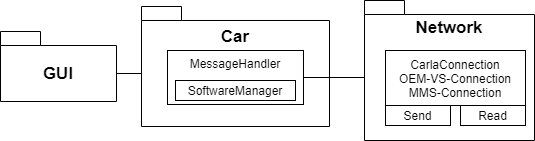
\includegraphics[width=0.8\columnwidth]{pictures/konzept-SAM.png}
	\label{img:sam}
	\caption{Architektur des Software Applikation Managers}
\end{figure}

\subsubsection{Architektur des OEM-Servers (Server)}
Die Architektur und auch die Funktionalität des Servers wurden unter der Beachtung des Uptane Standards geplant und implementiert. Die Architektur ist in Abbildung \hyperref[img:server]{16} dargestellt. Der Kern des Servers ist der \textbf{Director}, welcher eingehende Anfragen für Softwares abarbeitet. Der Director ist mit dem\textbf{ Image Repository} verbunden, in welchem sich die Softwares befinden, welche im Shop bereits bereitgestellt werden. Uptane gibt vor, eine \textbf{Inventory Database} zu führen, in welcher die Manifeste aller im Shop registrierter Fahrzeuge in der Form gespeichert sind, in welcher sie zuletzt von dem Director verifiziert wurden. Wird eine Anfrage an den Server geschickt, enthält diese das aktuelle Manifest des Fahrzeugs. Der Director vergleicht dieses mit dem Manifest, welches in der Inventory Database gespeichert ist. Durch den Vergleich des ByteCodes beider kann festgestellt werden, ob am Fahrzeug Änderungen von einer externen Instanz getätigt wurden oder nicht.
\begin{figure}[!h]
	\centering
	\includegraphics[width=0.75\columnwidth]{pictures/konzept-OEM-vs.png}
	\label{img:server}
	\caption{Architektur des Software Applikation Managers}
\end{figure}

%Abhängig von prototyp-version
Der Director kann eingehende Anfragen an den Software-User-Pattern-Recognizer\textit{(SUPR)} weiterleiten, welcher in Kapitel \hyperref[fs]{zwei} vorgestellt wurde. Der SUPR ist dafür zuständig, den Software-Bedarf von Fahrzeughaltern anhand ihrer Fahrdaten zu identifizieren. Er hat Zugriff auf das Image Repository und das \textit{Scenario Repository}. In diesem werden, wie in Kapitel \hyperref[konzept]{zwei} erwähnt, die zu einer Software hinzugefügten Szenarien gespeichert. Der Director leitet Anfragen weiter, die das feststellen von Softwarebedarf umfassen. Er selber verarbeitet nur die direkten Kaufanfragen für Software.

\subsection{Installation}
Die Installation der einzelnen Module muss muss getrennt voneinander passieren. Für die vollständige Nutzung muss sichergestellt sein, dass Carla auf dem PC auf welchem der Prototyp installiert werden soll lauffähig ist. Schauen Sie sich hierzu die Systemanforderungen von Carla an.  \footnote{\url{https://carla.readthedocs.io/en/latest/start_quickstart}, Aufgerufen am \today} Die einzelnen Module können auch auf getrennten Geräten genutzt werden, indem die IP-Adressen und Ports der Module über deren Config-Dateien angepasst werden. Die folgende Anleitung stellt dar, welche Schritte zur Installation der einzelnen Module getätigt werden müssen. Sie ist für Windowsgeräte ausgelegt und dauert ca. 30-40 Minuten.


\subsubsection{Server und SAM Installation}
\begin{itemize}
	\item[\textbf{1.}] \textbf{.zip-Ordner Herunterladen}\\
	Gehen Sie auf \url{https://github.com/hesty98/bachelorthesis}. Klicken Sie auf den \textit{"releases"}-Tab, welcher unter der Beschreibung des Repository zu finden ist.
	Laden Sie die Datei \textit{"prototyp.zip"} herunter und entpacken Sie den Ordner auf ihrem Laptop. In diesem Ordner finden Sie die .jar-Dateien mit welchen der Server und der SAM gestartet werden können. Der Ordner \textit{"PythonScriptsThesis"} wird später für die Installation von Carla benötigt.
	
	\item[\textbf{2.}] \textbf{IP-Adresse aufschreiben}\\
	Um das MMS und auch Carla mit dem Software Applikation Manager zu verbinden, müssen Sie ihre IP-Adresse kennen. Öffnen Sie hierzu ihr Windows-Temrinal und geben Sie \textit{ipconfig} ein. In der Zeile "IPv4-Adresse" steht ihre die IP-Adresse. Diese müssen Sie sich merken.
\end{itemize}


\subsubsection{MMS Installation}
\begin{itemize}
	\item[\textbf{1.}] \textbf{Android Studio herunterladen}\\
	Sie haben zwei Optionen, wie die Mensch Maschine Schnittstelle genutzt werden kann. Entweder sie simulieren das Android Gerät auf ihrem PC oder Sie installieren die App auf ein eigenes Tablett/Smartphone. Für beides wird eine aktuelle Version von Android Studio benötigt, die Sie hier \url{https://developer.android.com/studio} herunterladen können. Installieren Sie Android Studio und fahren Sie anschließend vor.

	\item[\textbf{2.}] \textbf{Code importieren}\\
	Das Repository der Mensch Maschine Schnittstelle liegt auf GitHub. Über Android Studio können Sie das Projekt direkt importieren. Klicken Sie hierfür auf "File" -> "new" -> "Project from Version control" -> "GitHub" und geben sie folgende URL ein: \url{https://github.com/hesty98/HMI}.\\
	
	\textbf{TESTEN}\\
	
	Alternativ kann das Projekt auch als .zip-Datei Heruntergeladen werden. Der extrahierte Ordner kann in Android Studio als Projekt geöffnet werden \textit{(File -> open -> Ordner wählen)}.
	
	\item[\textbf{3.}] \textbf{MMS Konfigurieren}\\
	Öffnen Sie in Android Studio die Datei Connection.java und passen Sie den Host entsprechend der IP des \textit{Software Applikation Managers} an. Die Datei befindet sich im 'network'-Ordner \textit{(app -> java -> com.linushestermeyer.hmi -> network)}.
	
	\item[\textbf{4.}] \textbf{MMS aufsetzen}\\
	Sie können die Mensch Maschine Schnittstelle nun entweder auf einem eigenen Gerät installieren oder das Gerät auf ihrem PC simulieren. Für beide Optionen Sie zuerst eine Konfiguration für die App erstellen.  Folgen Sie hierzu folgender Anleitung: \url{https://developer.android.com/studio/run/rundebugconfig}.
	
		\subitem \textbf{4.1 Eigenes Tablet}\\
			Zur Installation auf ihrem Tablet müssen Sie zunächst die \textit{Entwickler-Optionen} für dieses Freischalten und \textit{USB-Debugging} aktivieren. Folgen sie hierfür folgender Anleitung: \url{https://mobilsicher.de/ratgeber/usb-debugging-aktivieren}. Wurde dies getan, kann das Gerät an den PC angeschlossen werden. Über den grünen 'Play'-Button in der oberen Menuleiste kann die App auf Ihrem Gerät installiert werden.
			
		\subitem \textbf{4.2 Virtual Device}\\
			Wenn Sie Die App \textbf{nicht} auf einem eigenen Gerät installieren wollen, müssen sie mit Android Studio ein Simuliertes Gerät erstellen. Dies funktioniert nur, wenn ihr PC eine \textbf{Intel-CPU} hat, da Android Studio den \textit{HAXM-Service} von Intel zur Simulation nutzt. Verfügt ihr PC über eine Intel-CPUD, können Sie mit Hilfe folgender Anleitung ein Virtuelles Gerät erstelle: \url{https://developer.android.com/studio/run/managing-avds}. Erstellen Sie eine Instanz eines Tablets, nicht die eines Smartphone. \\
			Haben Sie ein \textit{VD} erstellt, können sie anschließend über den grünen 'Play'-Button in der oberen Menuleiste die App auf diesem Gerät installieren. 
\end{itemize}


\subsubsection{Carla Installation}
\begin{itemize}
	\item[\textbf{1.}] \textbf{Python installieren und SYS\_PATH hinzufügen}\\
	Damit Carla auf dem PC laufen kann, muss Python in Version 3.7 auf dem PC installiert sein und dem SYSTEM\_PATH hinzugefügt werden. Hierzu kann folgende Anleitung genutzt werden: \url{https://geek-university.com/python/add-python-to-the-windows-path/}. Hier die 3.4 nur durch eine 3.7 gedanklich ersetzen. Der PATH kann by der Installation auch durch das ankruezen einer Checkbox automatisiert werden.
	
	\item[\textbf{2.}] \textbf{Carla Herunterladen}\\
	Carla kann als .zip-Ordner Heruntergeladen werden. Die Dateien müssen in einen eigenen Ordner auf dem PC extrahiert werden. Als nächstes öffnen sie den Speicherort von Carla im Explorer und öffnen in diesem Fenster das Terminal \textit{(geben sie 'cmd' in den Suchbalken des Explorers ein)}. Jetzt müssen die für die Simulation notwendigen  Python-Packages \textit{pip, pygame und numpy} installiert werden. Die pip-Installation kann hier nachgelesen werden: \url{https://pypi.org/project/pip/}. Für die Installation von pip sollte zudem eine Adminsitrator-Konsole verwendet werden \textit{(Windows -> suche cmd' -> 'Als Administrator öffnen')}.Ist pip installiert, können mittels folgender Zeile die übrigen packages hinzugefügt werden:
	\begin{verbatim}
	py -3.7 -u pip install --user pygame numpy 
	EINFÜGEN HILFE
	\end{verbatim}
	Im Anschluss daran sollten Sie Carla ein mal testen. Starten Sie zunächst die Carla.exe und wechseln sie im Terminall in den PythonAPI/examples Ordner \textit{(cd PythonAPI/examples)}. Führen Sie anschließend folgenden Befehl durch:
	\begin{verbatim}
	py- 3.7 spawn_npc.py
	\end{verbatim}
	\item[\textbf{3.}] \textbf{Skripte einfügen}\\
	In der extrahierten .zip-Datei des SAM und Servers befindet sich ein Ordner mit dem Namen \textit{PythonScriptsThesis}. Kopieren Sie diesen Ordner in den \textit{PythonAPI}-Ordner von Carla und Sie haben es geschafft! 
	\item[\textbf{4.}] \textbf{Carla Konfigurieren}\\
	Abschließend sollten sie noch Konfigurationen an Carla vornehmen. Zuerst wird die Stadt geändert in welcher sich das Szenario abspielen wird. Hierzu\\
	\textbf{EINFÜGEN}\\
	
	Haben Sie die entsprechenden Werte eingetragen, speichern und schließen Sie die Datei. Anschließend wechseln sie in den Ordner \textit{PythonAPI/PythonScriptsThesis} und editieren Sie die install\_sw\_use\_service.py. Passen Sie die IP an die des \textbf{Software Applikation Managers} an. 
\end{itemize}

\subsection{Nutzung des Prototypen}
Die Module des Prototypen müssen in bestimmter Reihenfolge gestartet werden:
\begin{itemize}
	\item[\textbf{1.}]\textbf{Server}\\
	Server.jar ausführen.
	\item[\textbf{2.}]\textbf{Software Applikation Manager\\}
	SAM.jar ausführen
	\item[\textbf{3.}]\textbf{Carla\\}
	Starten Sie Carla. Führen Sie anschließend im Terminal im Ordner \textit{"PythonAPI/PythonScriptsThesis"} das Skript install\_sw\_use\_service.py aus.
	\begin{verbatim}
	py -3.7 install_sw_use_service.py
	\end{verbatim} 
	\item[\textbf{4.}]\textbf{Mensch Maschine Schnittstelle}\\
	Starten Sie die App auf ihrem Gerät oder in dem Virtual Device. Gehen Sie sicher, dass die App zuvor geschlossen war.
\end{itemize}
Im folgenden haben Sie fünf Bildschirme, über die alle Module des Prototypen sichtbar sind. Die Mensch Maschine Schnittstelle wartet auf eingehende Nachrichten, ebenfalls wie Carla. Die GUI des Software Applikation Managers ist in drei Bereiche aufgeteilt. Der Log auf Linken Seite stellt alle Ereignisse aus Sicht des Fahrzeugs dar. Der Log auf der Rechten Seite der GUI stellt sämtliche Ereignisse dar, die von dem Parkautomaten wahrgenommen werden. Zwischen beiden Logs sind diverse Knöpfe, die für die Steuerung des Prototypen gedacht sind.\\
$\underline{\textbf{Auto spawnen}}$ spawnt das Fahrzeug in der Carla Simulation. Mit den WASD-Tasten und der Maus können Sie herauszoomen und das Fahrzeug suchen. Prinzipiell ist es links vor ihnen. Der $\underline{\textbf{Zum Parkplatz fahren}}$-Knopf lässt das Fahrzeug in der Simulation zu einem Parkplatz fahren und es hält dort an.\\
Der $\underline{\textbf{In Erkennungsbereich fahren}}$-Knopf lässt das Fahrzeug in den Bereich fahren, in welchem der Parkautomat dieses erkennen kann. Nun kann sich der Parkautomat über den $\underline{\textbf{Sende Service Registrierung}}$-Knopf beim Fahrzeug registrieren. Der $\underline{\textbf{Sende ActionMessage}}$-Knopf sendet eine Nachricht an Carla, die entweder das Auto parken lässt oder es vom Parkplatz entfernen lässt. Das Szenario kann durch den $\underline{\textbf{Neustarten}}$-Knopf beliebig oft durchgeführt werden. Durch den $\underline{\textbf{Hack Car!}}$-Knopf wird das Auto "gehackt". Dies soll den Fall darstellen, wenn ein Fahrzeug versucht eine Software vom Shop zu installieren aber extern Änderungen im Auto vorgenommen wurden. Durch Änderungen am Fahrzeug verändert sich das Manifest des Fahrzeug, weshalb ein Fahrzeug keine Kommunikation mit dem Server aufbauen kann. Sämtliche Ereignisse die in Folge eines Knopfdrucks passieren, werden in den Logs notiert.\\\\
Über die \textbf{Mensch Maschine Schnittstelle} kann auf vom SAM verschickte Nachrichten reagiert werden. Initial ist der Home Screen des Shops zu sehen. Erhält das die MMS eine Software- oder ServiceRegistrationMessage, erscheint ein PopUp, in welchen der entsprechende Service bzw. die Software vorgestellt wird. Es kann entschieden werden, welches Angebot genommen werden soll oder auch die komplette Transaktion mit \textbf{Cancel} abgebrochen werden.

Die Server-GUI und die Simulation stellen weitere Visuelle Repräsentationen des Prototypen dar. In beiden können die Auswirkungen nachvollzogen werden, die durch die MMS und den SAM geschehen.

\subsection{Analyse des Prototypen und Ausblick auf die Weiterentwicklung}
Im Prototypen wurde die im Forschungsseminer erläuterte Uptane Architektur versucht grundlegend zu implementieren. Hierdurch konnte gezeigt werden, wie ein Fahrzeug in der Zukunft von externen Eingriffen geschützt werden könnte. Die erstellte Software Architektur lässt eine einfache Erweiterung des Prototypen zu. Für einen neuen Anwendungsfall muss bloß eine neue Software erstellt werden und das Carla Skript muss angepasst werden. Dies dauert ca. zwei Stunden. Die Installation des Prototypen ist relativ Zeitaufwendig und komplex, weshalb das Bereitstellen einer detaillierte Anleitung wichtig gewesen ist. \\

Der Prototyp hat dargestellt, wie eine Software über eine kabellose Schnittstelle orts- und zeitunabhängig gekauft und installiert werden kann. Zusätzlich wurde die Interaktion mit den in der Wertschöpfungskette identifizierten Service Providern implementiert, was zusätzliche Anwendungsfälle bieten kann. Über die GUIs kann nachvollzogen werden, was aktuell im Fahrzeug passiert und die Simulation kann ausreichend gesteuert werden. Die visuelle Repräsentation des Fahrzeugs in Carla unterstützt die Wirkung des Prototypen enorm, da der Betrachter direkt die Auswirkungen seiner Entscheidungen sieht. Auch die Interaktion über die Android-basierte Mensch Maschine Schnittstelle hat sich als sinnvoll erwiesen, da hierdurch ein guter Bezug zur Realität und Android Automotive gezogen werden kann. \\

Der Prototyp bietet noch eine Vielzahl an Erweiterungsmöglichkeiten. Der \textbf{Server} könnte um weitere Uptane-Funktionen erweitert werden. Die Erstellung eines Server-seitigen SUPR kann Türen öffnen, komplexe Suchalgorithmen auf der Basis von OpenScenario-Dateien in den Prototypen zu integrieren. Auch der \textbf{Software Applikation Manager} kann durch diverse neue Funktionen Sinnvoll erweitert werden. Ein Fahrzeug-basierter SUPR, dargestellt in Kapitel \ref{3.3}, kann Bestimmen von ein PopUp auf der MMS erscheinen soll und sodurch das wahllose erscheinen von PopUps verhindern. Die Steuerung über die GUI sollte den neuen Anwendungsfällen entsprechend angepasst werden, da nicht in jedem Anwendungsfall eine Kommunikation mit einem Service Provider stattfindet. Entfernt man sämtliche Nutzereingaben des Prototypen und automatisiert so die gesamte Simulation, können die dargestellten Anwendungsfälle beliebig hoch skaliert werden, wodurch ein Shop und die Zuverlässigkeit der Bereitstellung getestet werden kann.\\

Im Laufe der Entwicklung wurde deutlich, dass Carla äußerst umfangreich ist. Würden die Funktionen von Carla ausgereizt werden, könnte eine Vielzahl neuer Anwendungsfälle zum Prototypen hinzugefügt und in Carla visuell dargestellt werden. Auch eine wechsel zwischen autonomen Fahrfunktionen und eigenständiger Steuerung des Fahrzeugs kann in Carla erfolgen. Im aktuellen Prototypen ist Carla nur eine visuelle Repräsentation. Durch eine Implementierung des SAM in Python kann dies korrigiert werden und die Architektur kann um ein Modul verkleinert werden. Carla wäre dadurch sowohl die visuelle Repräsentation des Fahrzeugs als auch die "Business Logik".
\clearpage
\section{Resumé}
ergebnisse zusammenfassen\\
schlechtes\\
gutes\\
etc\\
Zusätzlich können normale apps immer heruntergeldaen werden. Die Besonderheit an Apps auf DriveAround ist, dass diese in das Fahrgeschehen eingreifen können.

\section{Ausblick}
weitere Anwendungsfälle, also erweiterung des Prototypen\\
SUPR als Projekt\\
Bedeutung User-Centered-Design im Kontext autonomer Fahrzeuge




\bibliographystyle{plain}
\bibliography{library}
\end{document}
